\typeout{NT FILE marrow_graph.tex}%

\chapter{Marrow-Graph}


In this chapter, we present the design and implementation of Marrow-Graph. We start by defining a programming model (section~\ref{sec:marrow_graph_programming_model}), then present the corresponding designed interface (section~\ref{sec:marrow_graph_interface}), and finally describe the implementation of the library, including its data structure (section~\ref{sec:marrow_graph_data_structure}), and the various supported operators (section~\ref{sec:marrow_graph_operators}) and algorithms (section~\ref{sec:marrow_graph_algorithms}).

%, a fast \gls{GPU}-accelerated dynamic graph processing library, which includes a set of commonly used graph processing algorithms and allows for efficient graph mutation.

\section{Programming Model}
\label{sec:marrow_graph_programming_model}

We will start by defining Marrow-Graph's programming model. Our goal while designing this model was to provide an interface that was as simple and expressive as possible. As discussed in Section~\ref{sec:programming_models},  bulk-synchronous is the most natural model for \gls{GPU} applications. More specifically, we believe that Gunrock's~\cite{paper:gunrock} programming model fits our purposes well. It allows one to highly optimize the small set of operations, and facilitate the development of algorithms utilizing these simple but fast operations. Another obvious benefit lies in the fact that Gunrock is an open-source project which already offers a wide array of algorithms implemented using this programming model.

Similarly to Gunrock~\cite{paper:gunrock}, Marrow-Graph provides two traversal operators: \textit{advance} and \textit{filter}. Both these operators map an input frontier to an output frontier, where a frontier consists of the IDs of a subset of the graph's vertices. As previously mentioned in Section~\ref{sec:gpu_graph_processing}, the compute operator can be fused together with the other traversal operators. So instead of having a dedicated compute operator, each transversal operator takes a compute function as input as well as any necessary compute arguments. The absence of a dedicated segmented intersection operator will be addressed later.

The filter operator has the following specifications:
%
\begin{displaymath}
\texttt{filter}(\text{Frontier} \: F, \: \texttt{FilterFun} \: f, \: \texttt{FilterArgs}... \: a) \: : \: \texttt{Frontier}
\end{displaymath}
%
where the first parameter $F$ is the input frontier composed by a set of vertex IDs. The second parameter $f$, is a function that acts both as the compute operator and the filter selector. This function is applied to every vertex $v$ referenced by $F$, and must return either 0 to exclude $v$ from the filtered frontier or return 1 to include $v$ in the filtered frontier. Any additional parameters of $f$, besides vector $v$, must be passed to the filter operator via the variadic arguments $a$. This allows the programmer to pass and process any auxiliary problem data. The output of the operator is frontier $F' \subset F$, containing only the vertex IDs corresponding to the vertices for which $f$ returned 1.

We now move on to the advance operator which has the following specification:
%
\begin{displaymath}
\texttt{advance}(\texttt{Frontier} \: F, \: \texttt{ComputeFun} \: c, \: \texttt{ComputeArgs}... \: a) \: : \: \texttt{Frontier}
\end{displaymath}
%
where, similarly to the filter operator, the first parameter is the input frontier composed by a set of vertex IDs. The second parameter $c$ expresses the compute function. This function is applied to every edge $e$ traversed during the advance operator, i.e. all the outgoing edges of the vertices referenced by the input frontier.
Given that vertex and edge information is stored separately in Marrow-Graph, $c$ must receive as parameters a source vertex $v_s$, a destination vertex $v_d$, and the edge $e$ connecting $v_s$ to $v_d$. 
Any additional parameters of $c$, besides $v_s$, $v_d$, and $e$, must be passed to the advance operator via the variadic arguments $a$. The output of the advance operator is a frontier $F'$ containing the IDs of all the unique neighbors of the vertices referenced by $F$.

% \begin{displaymath}
% \text{\textit{filter}}(\text{Frontier frontier}, \text{FilterFun fun}, \text{FilterArgs... args}) : \text{Frontier}
% \end{displaymath}

In Section~\ref{sec:gpu_graph_processing} we described the segmented intersection as an operator that can be applied over two frontiers. The latest versions of Gunrock however do not include a dedicated segmented intersection operator. Rather, a segmented intersection function, which can be invoked in the middle of a compute function, is provided. This means that the segmented intersection function can be applied over two vertices instead of two frontiers, i.e. it intersects the neighbors of the two vertices. Given that the compute function that is passed to the advance operator operates over edges composed of two vertices, the idea is that a segmented intersection can be executed during an advance. This is equivalent to performing a segmented intersection between a frontier $F$ and the frontier $F'$  obtained from performing an advance over $F$. According to Gunrock's authors, having such a segmented intersection function instead of a dedicated operator, is both more useful, and more efficient, given that we can perform an advance and a segmented intersection simultaneously.  We decided to follow the same philosophy and incorporate a segmented intersection function which can be invoked in the middle of an advance's compute function $c$. The segmented intersection function has the following specification: 
%
\begin{displaymath}
\texttt{segint}(\texttt{Graph} \: g, \texttt{Vertex} \: v_a, \: \texttt{Vertex} \: v_b, \: \texttt{IntersectFun} \: t, \: \texttt{IntersectArgs}... \: a) \: : \: \texttt{int}
\end{displaymath}
%
where the first parameter includes the graph data required to perform the intersection (more on this later). The second and third parameters $v_a$ and $v_b$ correspond to the vertices to intersect. The fourth parameter $t$ is a function that allows the user to express some logic to be performed over each intersection (we will later see that some algorithms require this). Function $t$ must receive as parameters the two vertices being intersected $v_a$ and $v_b$, and the intersected vertex $v_i$. Any additional arguments can be passed using the variadic arguments $a$. The output of the segmented intersection function is an integer representing the total number of intersections between $v_a$ and $v_b$.

\section{Interface}
\label{sec:marrow_graph_interface}

\begin{listing}%[t]
\begin{minted}
[
frame=lines,
linenos,
fontsize=\scriptsize
]
{cpp}
template<typename vertex_attributes>
struct vertex {
    idx_t idx;
    std::size_t degree;
    idx_t adjacency_list;
    idx_t adjacency_list_end;
    vertex_attributes attributes;
};

template<typename edge_attributes>
struct edge {
    idx_t dst;
    edge_attributes attributes;
};

template <typename vertex_attributes, typename edge_attributes>
class graph {

    using Vertex = vertex<vertex_attributes>;
    using Edge = edge<edge_attributes>;

    idx_t add_vertex(vertex_attributes attributes) ;
    bool remove_vertex(idx_t idx) ;
    bool add_edge(idx_t src, idx_t dst, edge_attributes attributes) ;
    bool add_edge_batch(edge_insertion_batch<edge_attributes>& batch) ;
    bool remove_edge(idx_t src, idx_t dst) ;
    bool remove_edge_batch(edge_deletion_batch<edge_attributes>& batch) ;
    bool edit_edge(idx_t src, idx_t dst, idx_t new_dst) ;
    vector<idx_t> get_connection(idx_t idx) ;
    std::size_t get_degree(idx_t idx) ;
    std::size_t get_number_of_vertex() ;
    std::size_t get_number_of_edges() ;
    void sort() ;

    template <bool return_frontier = true, bool balanced = true>
    template <typename compute_fun, typename... compute_args>
    vector<idx_t> advance(vector<idx_t>& frontier, compute_fun& cfun, compute_args&... cargs);
    
    template <typename filter_fun, typename... filter_args>
    vector<idx_t> filter(vector<idx_t> &frontier, filter_fun& ffun, filter_args&... fargs);
};
\end{minted}
\center
\caption{Graph interface.}
\label{lst:graph_interface}
\end{listing}

% Graph abstraction
% abstraction  allows for the future experimentation with different data structures
% templated vertex attributes and templated edge attributes

We now present Marrow-Graph's interface that implements the previously described programming model and also provides a set of graph manipulation operations (the complete C++ abstract class can be found in Listing~\ref{lst:graph_interface_complete} of Appendix~\ref{app:listings}). Graphs represented in Marrow-Graph are directed and optionally weighted (using the optional attributes). As we can see in Listing~\ref{lst:graph_interface}, three structs are provided. The \texttt{vertex} struct includes a vertex's ID, its degree, pointers to the start and end of its adjacency list, and a templated field for storing custom vertex attributes. The \texttt{edge} struct includes the ID of the destination vertex (the source vertex is implied) and a templated field for storing custom edge attributes. Finally, the \texttt{graph} class offers a set of methods for manipulating and queering the graph, as well as the advance and filter operators.

%\paragraph{\textbf{Updates}.}
Regarding graph manipulation functions, we offer a method to create a new vertex \texttt{add\_vertex} which returns the ID of the generated vertex. Then using the generated IDs, the user can invoke the methods \texttt{remove\_vertex}, \texttt{add\_edge}, \texttt{remove\_edge}, and \texttt{edit\_edge}. Additionally, an \texttt{add\_edge\_batch} method and a \texttt{remove\_edge\_batch} method are provided to perform optimized insertions and deletions of batched edges. As seen in Listing~\ref{lst:edge_insertion_batch}, an edge batch is composed by a \texttt{std::map}, whose key is the ID of a source vertex, and value is a vector of outgoing edges. This allows Marrow-Graph to perform edge insertions and deletions optimally by iterating over consecutive edges that share the same source vertex.



\begin{listing}[t]
\begin{minted}
[
frame=lines,
linenos,
fontsize=\scriptsize
]
{cpp}
template<typename edge_attributes>
struct edge_insertion_batch {
    std::size_t size;
    std::map<idx_t, std::vector<edge<edge_attributes>>> edges;

    void add(idx_t src, idx_t dst, edge_attributes attributes);
};
\end{minted}
\center
\caption{Edge insertion batch.}
\label{lst:edge_insertion_batch}
\end{listing}

\subsection{Operators}
\label{sec:marrow_graph_interface_operators}

%\paragraph{\textbf{Operators}.}
%Similarly to Gunrock~\cite{paper:gunrock}, Marrow-Graphprovides four main operators: advance, filter, compute and segmented intersection. As previously mentioned~\ref{gpu_graph_processing}, the compute operator can be used together with the other traversal operators. For this reason, instead of having a dedicated compute operator, each transversal method takes a compute operator as input as well as any necessary compute arguments. Besides the compute operator, all the operators receive an input frontier and return the corresponding result frontier. These frontiers are represented as a Marrow vector of vertex IDs. The absence of a dedicated segmented intersection operator will be discussed later.

As discussed previously in Section~\ref{sec:marrow_graph_programming_model}, the advance and filter operators operate over frontiers and parameterized functions. To express these concepts in Marrow-Graph's interface, we use \texttt{marrow::vector}s of IDs to represent the former, and resort to templated functors and variadic templated arguments for the latter. Note that even though in Listing~\ref{lst:graph_interface} the advance and filter operators have a return type \texttt{vector<idx\_t>} to make it clear that these functions return a new frontier, in the actual implementation of Marrow-Graph, these functions have \texttt{auto} as their return type. This allows Marrow to return an expression that evaluates to the desired container, rather than returning the actual container. This is of course much more efficient, given that containers are heavier objects than Marrow expressions.

\paragraph{\textbf{Advance}.}
The \texttt{advance} method (Lines~35 to 37 of Listing~\ref{lst:graph_interface}) receives as input a templated compute function and its corresponding arguments (expressed with a variadic template). The \texttt{compute\_fun} type must be a functor whose function call operator \texttt{()} adheres to the following signature: \[\texttt{void operator()(Vertex\& sv, Vertex\& dv, Edge\& e, Args\&... a) \{ ... \}}\] As specified by our model, the advance's compute function describes an operation that is performed over a single 
edge traversed during advance. Marrow-graph ensures that this function is actually applied over all the outgoing edges of the input frontier. The parameters \texttt{sv}, \texttt{dv} and \texttt{e} represent a single outgoing edge: \texttt{sv} contains the data and attributes of the source vertex, \texttt{dv} contains the data and attributes of the destination vertex, and \texttt{e} contains the attributes of the edge connecting these vertices. Besides these three arguments, the compute function can also receive and operate over any number of auxiliary arguments. These arguments must either be basic data types, Marrow containers or \texttt{result} wrapped Marrow containers. If the compute function changes the state of a Marrow container, it can be passed to the advance operator using the \texttt{result} wrapper, informing Marrow-Graph that the container is a result that is computed on the device. We will discuss this in more detail in section~\ref{sec:host_dev_sync}. Note however, that although the auxiliary arguments we pass to the \texttt{advance} function can be Marrow containers, the type of the arguments of the \texttt{cfun} function must be their kernel type counterparts, similarly to how we define and use Marrow functions. For example, we might pass a \texttt{vector<int>} as an auxiliary argument to advance, but receive a \texttt{int*} in the \texttt{cfun}. Given that the advance operator is executed on the device, the device code must operate over basic data type pointers rather than complex Marrow containers.

While developing Marrow-Graph, we found out that some algorithms use the advance operator without requiring the resulting advanced frontier. These algorithms only require the compute operator to be applied over all outgoing edges. For this reason, the \texttt{compute} function has an additional \texttt{return\_frontier} template (set to true by default), which can be set to false, in order to run an optimized version of the operator which returns an empty frontier. Besides the \texttt{return\_frontier} template, we can see that there is also a \texttt{balanced} boolean template. This template only has an effect whenever \texttt{return\_frontier} is set to false, allowing the optimized advance operator to run either in a balanced or unbalanced manner. We will further discuss this in Section~\ref{sec:advance_operator}.



\begin{listing}[t]
\begin{minted}
[
frame=lines,
linenos,
fontsize=\scriptsize
]
{cpp}
struct vertex_attribute {};
struct edge_attribute { int weight; };

struct compute_total_weight_fun {
    marrow_function
    void operator()(Vertex &src, Vertex &dst, Edge &edge, int* weights) {
        marrow::atomic::add(&weights[dst.idx], edge.weight);
    }
};

graph<vertex_attribute, edge_attribute> g = ...;
vector<int> weights(g.get_number_of_vertex());
fill(weights, 0);

idx_t vertex_id = ...;
vector<idx_t> frontier = { vertex_id };
vector<idx_t> advanced_frontier = g.advance(frontier, compute_total_weight_fun(), result(weights));
int total_weight = reduce<plus>(weights);
\end{minted}
\center
\caption{Advance example.}
\label{lst:advance_example}
\end{listing}

Listing~\ref{lst:advance_example} shows an example of how the advance operator might be used to compute the sum of the weights of all the outgoing edges of a given vertex. For the sake of simplicity, we will assume this graph has not been subjected to vertex deletions which could affect the required size of the \texttt{weights} container. In Lines~11-13 we start by instantiating a graph \texttt{g} and a vector \texttt{weights} with all values initialized to 0. In Lines~15-16 we define a frontier with a single vertex (the vertex whose neighbor weights we will be summing). In Line~17 we call the \texttt{advance} operator over the frontier, passing it an instance of the \texttt{compute\_total\_weight\_fun} functor and the \texttt{weights} vector. Looking at Lines~4-9, we can see that this functor follows the previous signature rules, and atomically sums an edge's weight to the \texttt{weights} array at the index corresponding to the destination vertex. This means that after the advance operator finishes, \texttt{weights} will contain all the weights of the outgoing edges in the corresponding positions of the destination vertices. All the other positions of the container will remain equal to 0. Finally, In Line~18 we sum all the values of \texttt{weights} with a Marrow reduce, and obtain the total sum of weights. You may have noticed that instead of passing the \texttt{weights} vector directly in Line~17, we actually pass \texttt{result(weights)}. As previously mentioned, this informs Marrow-Graph that the \texttt{weights} argument is a result that is computed during the \texttt{compute} function.

\paragraph{\textbf{Filter}.}
The \texttt{ffun} parameter and corresponding \texttt{fargs} parameter from the filter method (Lines~39 to 40 of Listing~\ref{lst:graph_interface}) follows similar restrictions to the previously discussed compute function and arguments. The main difference is that filter does not operate over edges, but rather directly over the vertices of the input frontier. Therefore, the \texttt{filter\_fun} type must be a functor whose function call operator \texttt{()} receives a single vertex as input and any number of auxiliary arguments: \[\texttt{int operator()(Vertex\& v, Args\&... a) \{ ... \}}\] Additionally, the return type of the operator must be an integer, instead of void, to allow one to express the filter selection logic described by our model. 

Listing~\ref{lst:filter_example} shows how the filter operator can be used to filter-out inactive vertices from a frontier. In this example, we define a graph whose \texttt{vertex\_attributes} includes a \texttt{active} field. In Line~13 we apply the filter operator over an input frontier and pass it an instance of the \texttt{remove\_inactive\_fun} functor. This functor returns 1 if the input vertex is active and 0 otherwise. This means that the filter operator will return a frontier that only includes the vertices that have the \texttt{active} field set to 1.

\begin{listing}[t]
\begin{minted}
[
frame=lines,
linenos,
fontsize=\scriptsize
]
{cpp}
struct vertex_attribute { char active = 1; };
struct edge_attribute {};

struct remove_inactive_fun {
    marrow_function
    void operator()(Vertex &v) {
        return v.active ? 1 : 0;
    }
};

graph<vertex_attribute, edge_attribute> g = ...;
vector<idx_t> frontier = { ... };
vector<idx_t> filtered_frontier = g.filter(frontier, remove_inactive_fun());
\end{minted}
\center
\caption{Filter example.}
\label{lst:filter_example}
\end{listing}

\paragraph{\textbf{Segmented Intersection}.}
%
In order to provide the segmented intersection specified by our model, we defined a marrow function (that can be invoked in the middle of a compute function that is executed on the device) whose signature can be seen in Listing~\ref{lst:segmented_intersection_function}. The function returns an integer with the number of intersections and receives as input: a graph struct, the two intersecting vertices, and a \texttt{on\_intersection\_fun} alongside its \texttt{on\_intersection\_arguments}. The graph struct \texttt{graph\_bal\_t} found in the code snippet, is specific to the blocked adjacency graph implementation. In the future, this struct can easily be templated to provide a more generic function that supports multiple implementations. Regardless, although this parameter is required to compute the intersection, it can be mostly ignored by the user. As stated before, even though the function returns the total number of intersections, some algorithms require performing some logic for each intersection. This is done via the \texttt{on\_intersection\_fun}. The \texttt{on\_intersection\_fun} type must be a functor whose function call operator \texttt{()} adheres to the following signature: \[\texttt{void operator()(Vertex\& va, Vertex\& vb, Vertex\& vi, Args\&...) \{ ... \}}\] Like our model specifies, this function operates over a single intersection, and its then Marrow-Graph's job to ensure this method is called for every intersection. Parameters \texttt{va} and \texttt{vb} represent the two vertices being intersected, while \texttt{vi} represents the intersected vertex (a neighbor that \texttt{va} and \texttt{vb} have in common).

 \begin{listing}[t]
\begin{minted}
[
frame=lines,
linenos,
fontsize=\scriptsize
]
{cpp}
template<typename vertex_attributes, typename edge_attributes, 
    typename on_intersection_fun, typename... on_intersection_arguments>
marrow_function
int segmented_intersection(graph_bal_t<vertex_attributes, edge_attributes> &graph,
    vertex<vertex_attributes>& vertex_a,
    vertex<vertex_attributes>& vertex_b,
    on_intersection_fun& on_intersection,
    on_intersection_arguments&... on_intersection_args);
\end{minted}
\center
\caption{Segmented intersection function.}
\label{lst:segmented_intersection_function}
\end{listing}

Listing~\ref{lst:segmented_intersection_example} shows how the segmented intersections function can be used to compute the total number of intersection between the vertices of a frontier $F$ and its advanced frontier $F'$. In Lines~16-19 we define a graph, a vector to store intersection counts, and a frontier. In Line~20 we apply the advance operator over the frontier passing it an instance of a \texttt{compute\_intersection\_count\_fun} functor and all the necessary arguments, including an instance of the \texttt{on\_intersection\_fun}. The \texttt{vertex\_intersection\_count} is wrapped as a \texttt{result} since it is a result manipulated by the compute function.  In this example, since we do not want to perform any logic for each intersection, the body of the \texttt{on\_intersection\_fun} functor can stay empty. Note that our compute function defined In Lines~7-14 has a slightly different signature than the one we established before. The difference is the first parameter \texttt{graph}. Given that it is mandatory to pass this struct to the \texttt{segmented\_intersection} function, a Marrow-Graph compute function can optionally contain the graph struct as its first parameter. In Line~11 we call the \texttt{segmented\_intersection} function passing it the graph struct, the source and destination vertices (which are provided to any advance's compute functor), and the \texttt{on\_intersect} functor. The result is stored in a local variable \texttt{nintersections}. In Line~12 we atomically add the intersection count to the \texttt{vertex\_intersection\_count} container in the corresponding index of destination vertex. Finally, in Line~22, we compute the total intersection count with a Marrow reduction over the \texttt{vertex\_intersection\_count} vector.

\begin{listing}
\begin{minted}
[
frame=lines,
linenos,
fontsize=\scriptsize
]
{cpp}
struct on_intersection_fun {
    marrow_function
    void operator()(Vertex& vertex_a, Vertex& vertex_b, Vertex& intersection_vertex) {
    }
};

struct compute_intersection_count_fun {
    marrow_function
    void operator()(Graph& graph, Vertex &src, Vertex &dst, Edge &edge, 
        int* vertex_intersection_count, on_intersection_fun& on_intersect) {
        int nintersections = segmented_intersection(graph, src, dst, on_intersect);
        marrow::atomic::add(&vertex_intersection_count[dst.idx], nintersections);
    }
};

graph<vertex_attribute, edge_attribute> g = ...;
vector<int> vertex_intersection_count(g.get_number_of_vertex());
fill(vertex_intersection_count, 0);
vector<idx_t> frontier = { ... };
vector<idx_t> advanced_frontier = g.dvance(
    frontier, compute_intersection_count_fun(), result(vertex_intersection_count), on_intersection_fun());
int total_intersection_count = reduce<plus>(vertex_intersection_count);
\end{minted}
\center
\caption{Segmented intersection example.}
\label{lst:segmented_intersection_example}
\end{listing}


Similarly to Gunrock, in order to achieve an efficient and fast implementation of the \texttt{segmented\_intersection} function, it is assumed that the adjacencies of the intersecting vertices $v_a$ and $v_b$ are sorted. The motives for this are discussed in Section~\ref{sec:segmented_intersection}. If a user wants to ensure that these adjacencies are sorted before performing a compute with a segmented intersection, the \texttt{sort} function (Line~33 of Listing~\ref{lst:graph_interface}) can be invoked. Additionally, for the blocked adjacency graph implementation, when initializing a graph, the user can specify that the graph should track unsorted adjacency lists. This adds some slight overhead to the graph manipulation functions, but improves the \texttt{sort} function performance drastically, as it only sorts the adjacency lists that might have become unsorted.
% Assuming sorted adjacencies we can achieve a  segmented intersection with a time complexity of $O(n)$, with $n$ equal to the sum of the degrees of $v_a$ and $v_b$. Otherwise 

\section{Data Structure}
\label{sec:marrow_graph_data_structure}

%Design and Implementation (including manipulations)

We will now discuss the data structure chosen for the internal implementation of Marrow-Graph. We decided to base our data structure on FaimGraph~\cite{paper:faimgraph}, as it has proven to be a versatile yet highly efficient data structure for storing dynamic graphs. FaimGraph is comprised by a vertices vector, a set of blocked adjacency lists, and two deleted index queues as seen in Figure~\ref{fig:faimgraph_data_structure}. In Marrow-Graph, we use the same sub-data structures, with the addition of two index vectors storing the links between blocks. Figure~\ref{fig:mg2_data_struct} shows a representation of the data structure indicating each corresponding Marrow collection.  

The vertices are stored using a \texttt{marrow::vector} of \texttt{vertex}s. We chose a Marrow vector, given that vertices must be accessible both on the host, to perform updates and query the graph, and on the device, to execute the operators. Additionally, the vector data structure allows for insertions and deletions of vertices. 

The adjacencies are stored using a \texttt{marrow::vector} of fixed size \texttt{marrow::array}s of \texttt{edge}s. Each edge stores the destination vertex and optional attributes. Given that the adjacency lists are supposed to be stored using fixed-size blocks, the most fitting container is a variable-sized Marrow vector of fixed-sized arrays. This way, we can easily insert and remove new blocks as needed, and still achieve good memory locality given that consecutive blocks (or arrays in this case) will be stored contiguously in memory. Similarly to the vertices, we use a Marrow container instead of a \texttt{std} container, since the adjacency lists must be accessible both on the host and on the device.

Block links are stored using \texttt{marrow::vector}s of indexes. Once again, a Marrow vector allows us to insert and delete new block links whenever a block is added or removed and makes the container accessible both on the host and device. The advance operator requires the block links to be accessible on the device in order to iterate over the adjacency lists comprised of multiple blocks.

Finally, the deletion queues are stored with basic \texttt{std::queue}s. We do not use Marrow containers as the deletion queues are only accessed on the host (all graph updates are performed on the host). 


 \begin{listing}
\begin{minted}
[
frame=lines,
linenos,
fontsize=\scriptsize
]
{cpp}
template<typename vertex_attributes, typename edge_attributes, std::size_t block_size>
class graph_bal : public graph<vertex_attributes, edge_attributes> {
    ...
    std::size_t nvertex = 0;
    std::size_t nedges = 0;
    vector<vertex<vertex_attributes>> vertices;
    vector<array<edge<edge_attributes>, block_size>> blocks;
    vector<idx_t> block_links;
    vector<idx_t> block_links_reversed;
    std::queue<idx_t> deleted_vertices;
    std::queue<idx_t> deleted_blocks;
    bool track_unsorted_adjacencies;
    std::set<idx_t> unsorted_adjacency_lists;
}
\end{minted}
\center
\caption{graph\_bal fields.}
\label{lst:graph_bal}
\end{listing}


\begin{figure}[t]
  \centering
    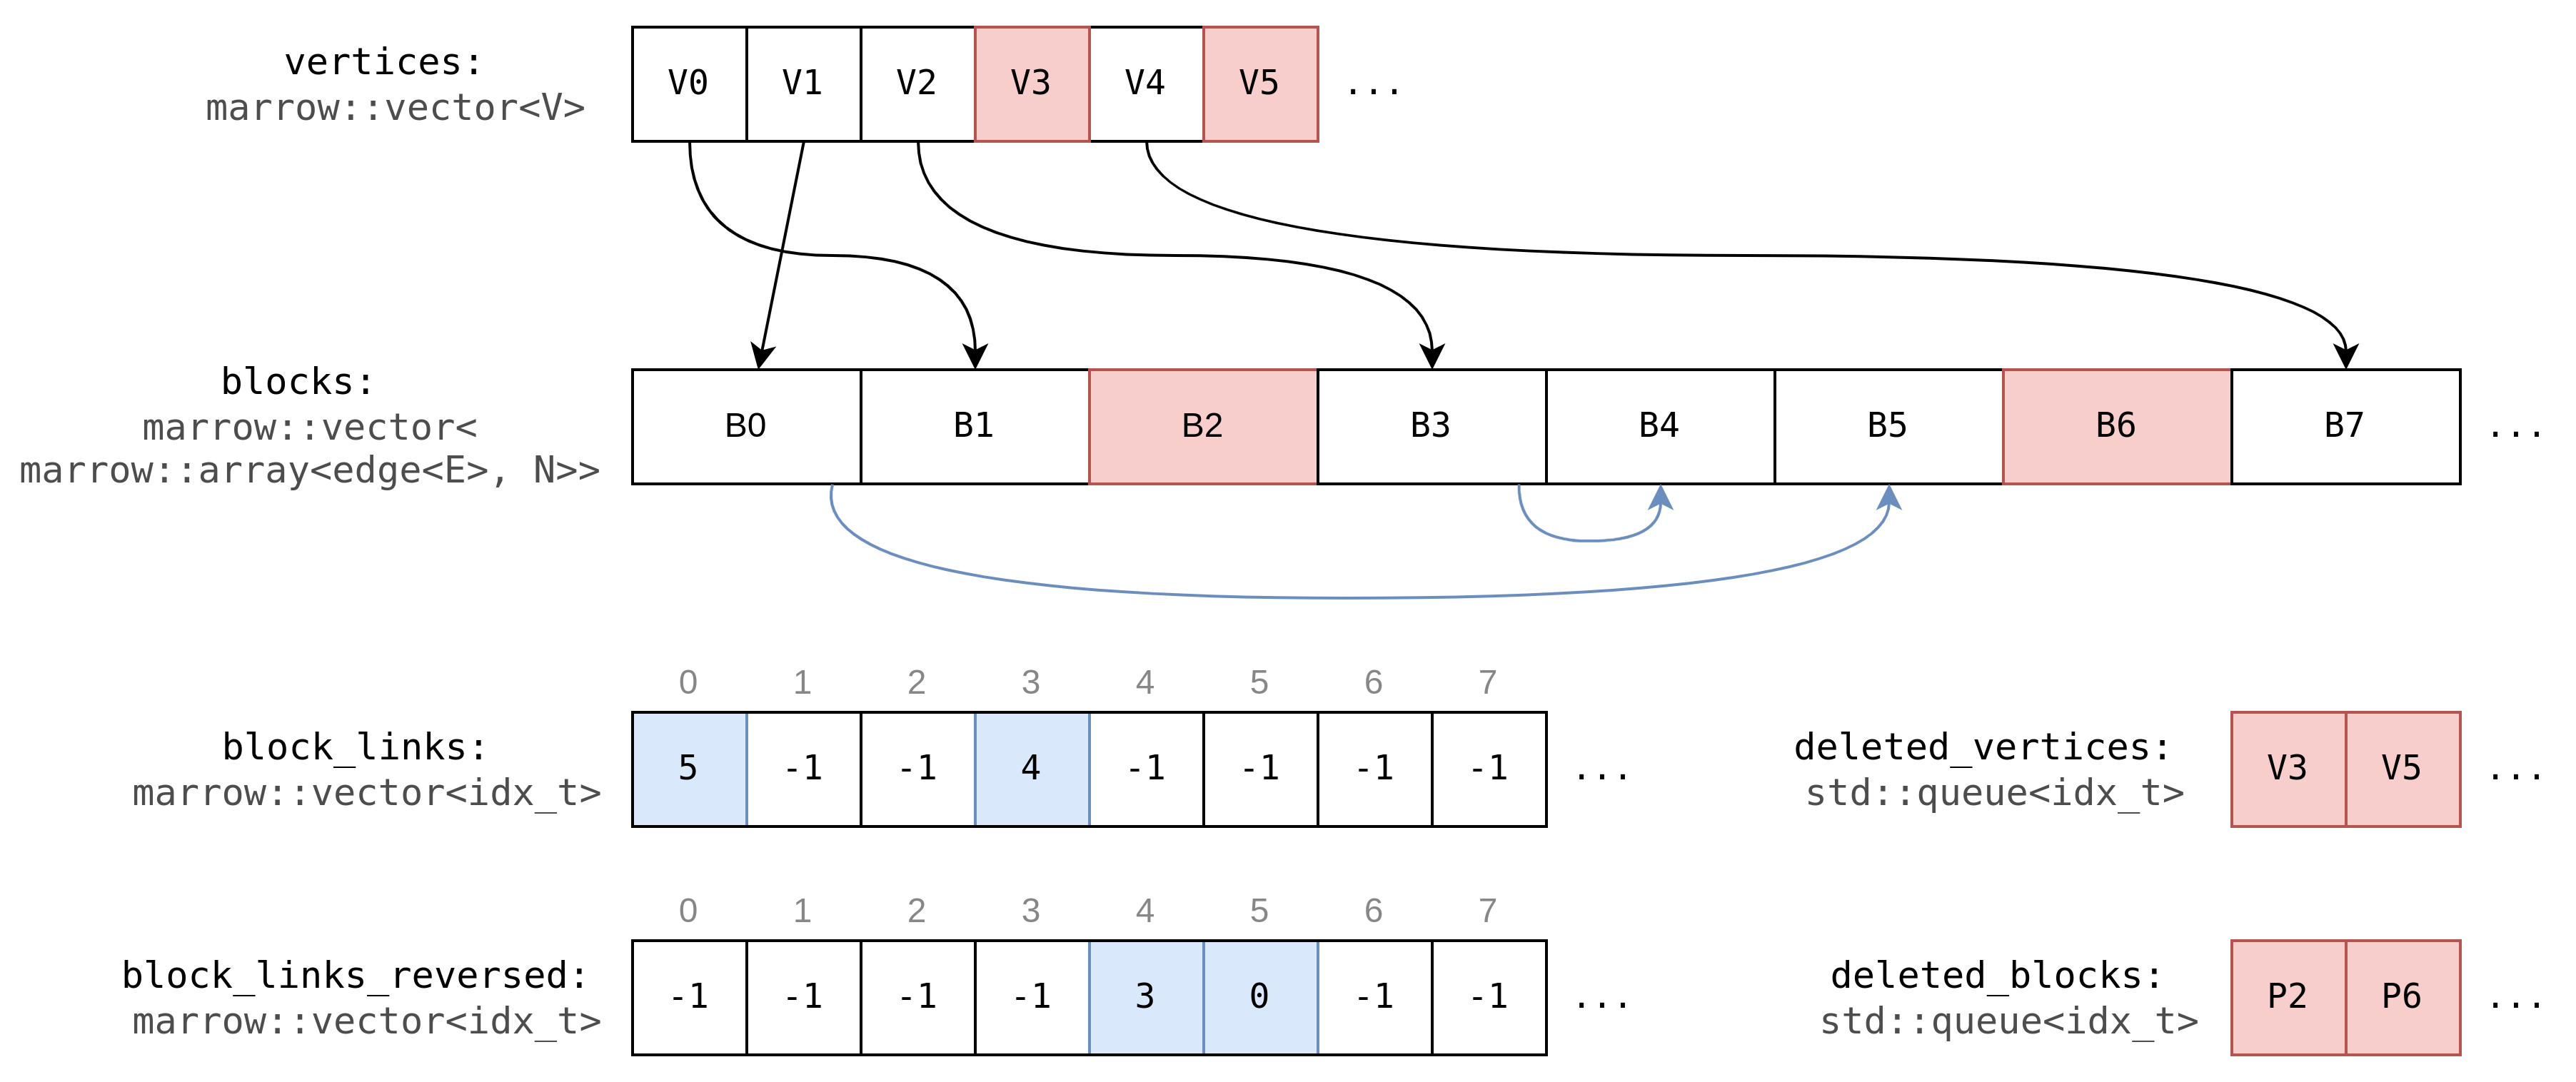
\includegraphics[width=\textwidth]{Chapters/Figures/Images/marrow_graph_data_struct.png}
    \caption{Marrow-Graph's data structure.}
\label{fig:mg2_data_struct}
\end{figure}

Listing~\ref{lst:graph_bal} shows the actual class and fields used to define the \gls{BAL} implementation of Marrow-Graph. Besides the aforementioned data structures, two counters \texttt{nvertex} and \texttt{nedges} are also included to keep track of the total number of vertices and edges in the graph, and a \texttt{unsorted\_adjacency\_lists} set is used to track unsorted adjacency lists. If a graph is flagged to track unsorted adjacencies, whenever edges are inserted or deleted, Marrow-Graph verifies if the corresponding adjacency list becomes unsorted, and if it does, the adjacency list's source vertex ID is added to the \texttt{unsorted\_adjacency\_lists} set. We will see in Section~\ref{sec:marrow_graph_sorting} how this allows for more efficient graph sorting.

In terms of indexing, each element of the \texttt{vertices} vector stores an index to the first and last adjacency blocks. The \texttt{block\_links} and \texttt{block\_links\_reversed} vectors can then be used to traverse the blocked adjacency lists in either direction. Looking at Figure~\ref{fig:mg2_data_struct} we can see that, for example, vertex \texttt{V1} has an adjacency list that starts at block \texttt{B0} and ends at block \texttt{B5}. Looking at the \texttt{block\_links} container, we can see that indeed the link at position 0 stores the index 5. Then the link at position 5 stores the index -1. A value of -1 indicates that there does not exist another link, i.e. the adjacency list ends.

\subsection{Host-Device Synchronization}
\label{sec:host_dev_sync}

Initially, the graph is solely stored on the host. Once an operator (advance or filter) is invoked, all the necessary containers are allocated and synchronized to the device. Given that the operators are implemented using Marrow functions and Marrow skeletons, this allocation and synchronization is ensured naturally by Marrow. All graph manipulations (adding, removing, and editing edges and vertices) are performed on the host. Once again, Marrow tracks any changes and synchronizes the dirty containers automatically whenever an operator is executed.


\begin{figure}
  \centering
    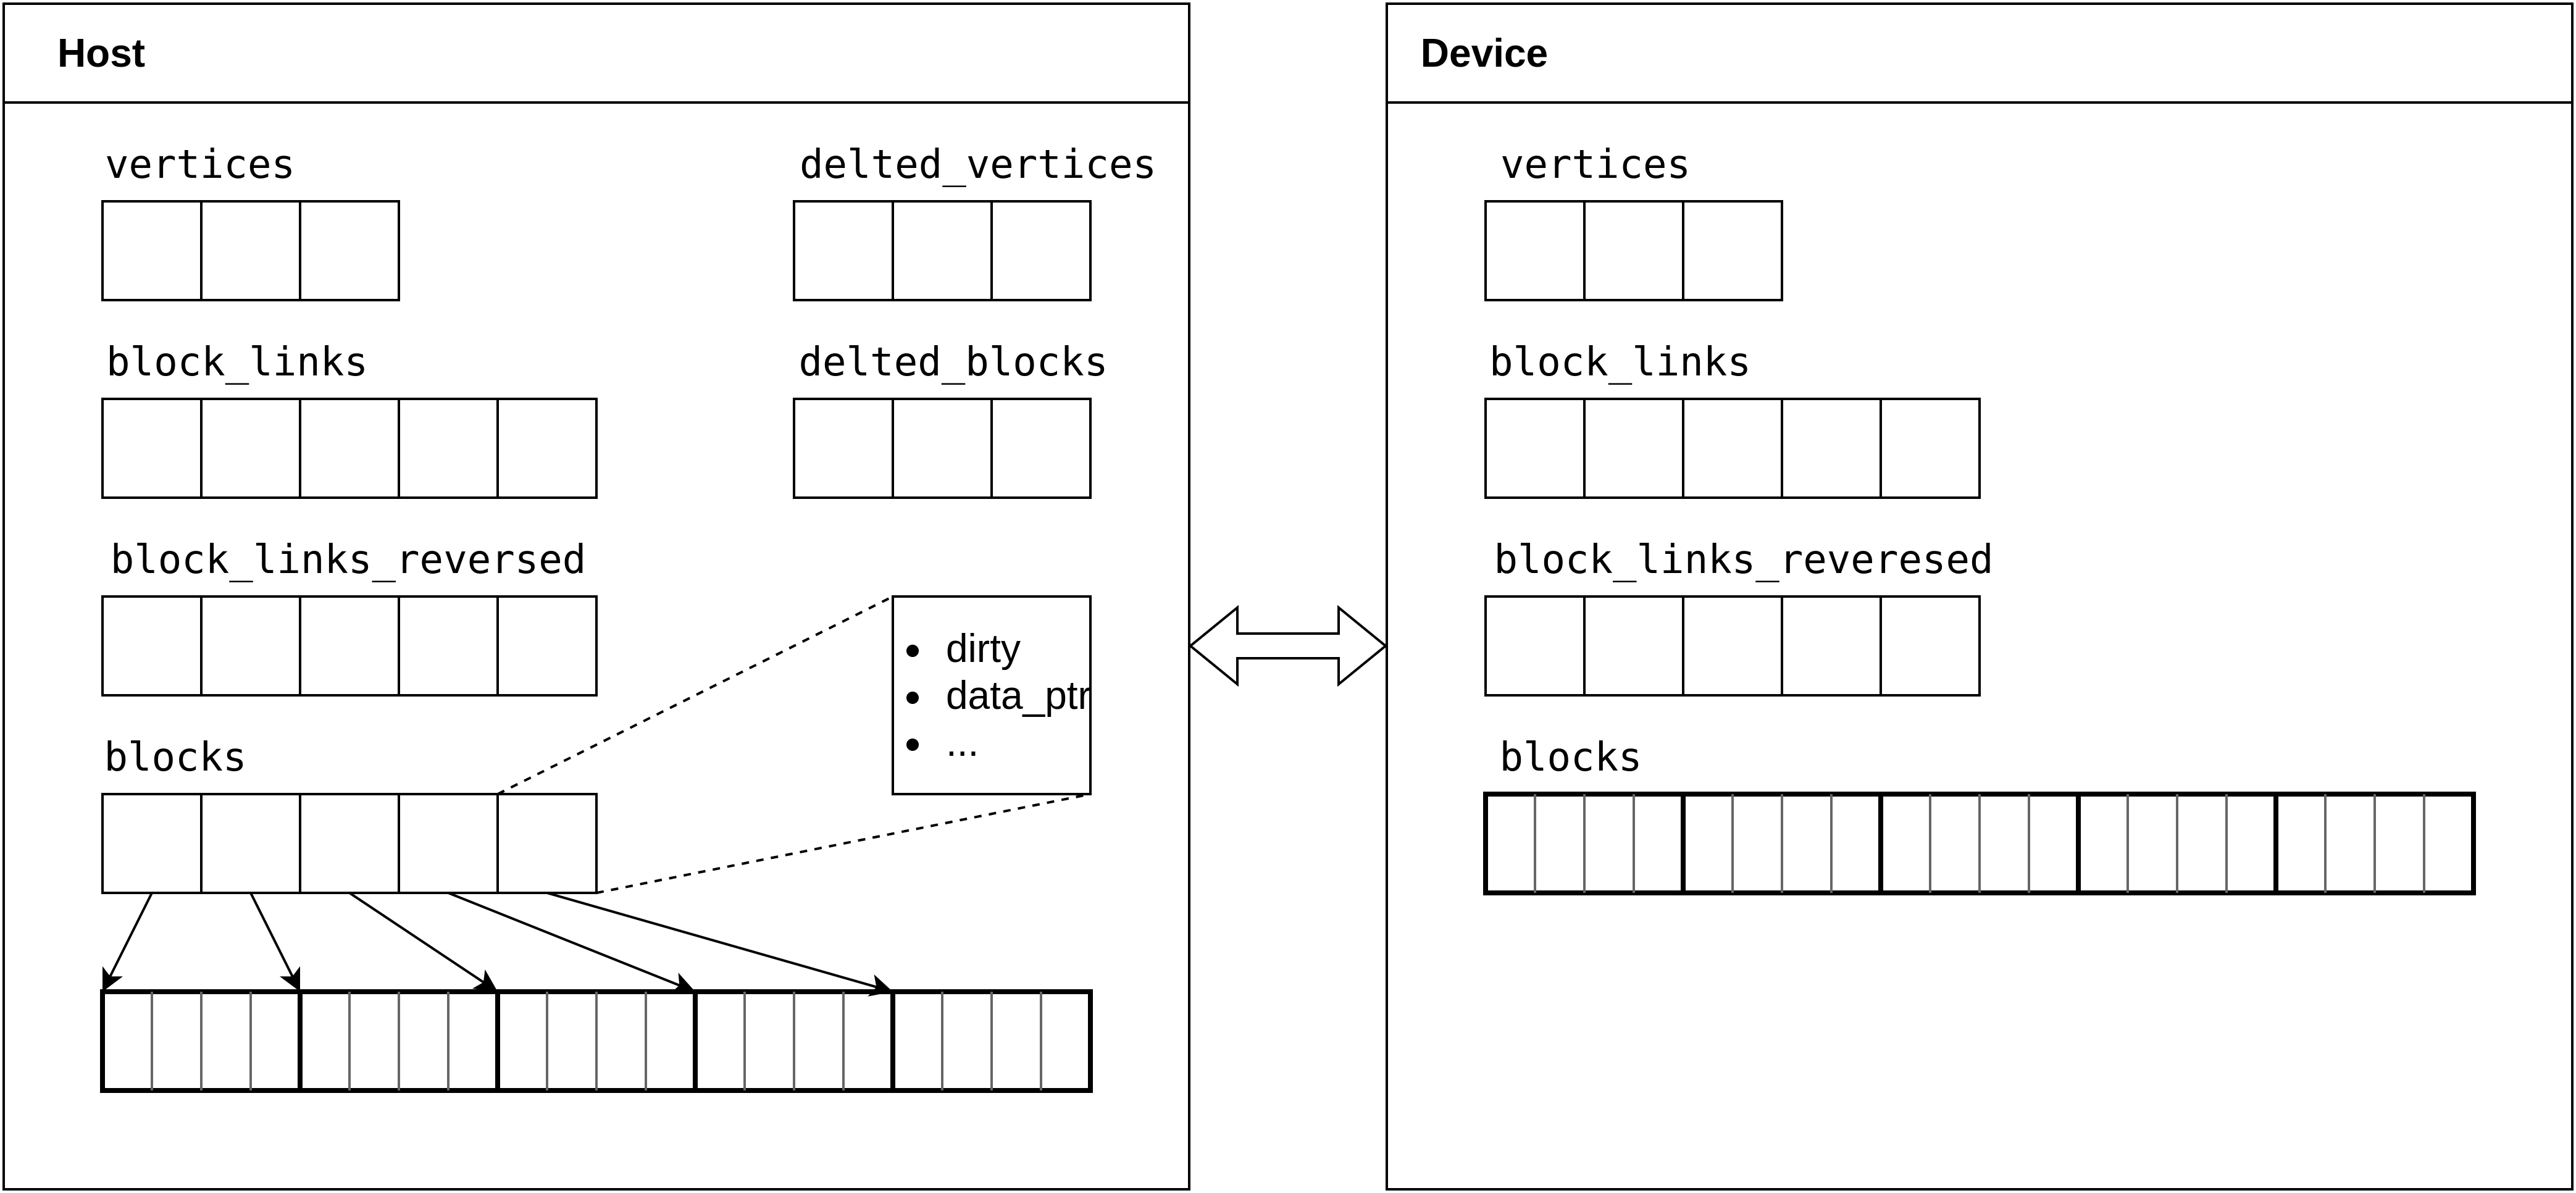
\includegraphics[width=\textwidth]{Chapters/Figures/Images/host_device_memory.png}
    \caption{Host/device memory layout.}
\label{fig:host_device_memory}
\end{figure}

% TODO: describe vector<array>: Single continuous block of data on device, single block of continuous data on host + vector of arrays with metadata. Only dirty arrays are synched

Figure~\ref{fig:host_device_memory} shows the memory layout once a graph has been loaded and synchronized with the \gls{GPU}. As we can see, most containers are simply stored as contiguous vectors on the host, and have a replica stored on the device. One more nuanced container is the \texttt{vector<array<N,T>\!>}, which we use to store blocks (or adjacencies). Assuming a fixed array size of $N$ and a variable vector size of $S$, a \texttt{vector<array<N,T>\!>} is stored on the host using two data structures. A contiguous block of data of length $N*S$, and a vector of Marrow arrays of length $S$. These arrays only contain metadata and point to the contiguous memory block. This allows user-friendly manipulations of the data structure on the host while allowing for efficient memory transfers and memory accesses to/on the device. If the host would only store a vector of arrays containing the data, transferring the whole vector to the device would require $N$ separate memory transfers, rather than a single large memory transfer of $N*S* \text{sizeof} (T)$ bytes. The vector of arrays that we store on the host, also allows Marrow to track singular dirty arrays. When Marrow synchronizes the vector to the device, if it's been already allocated, only the dirty arrays are synchronized, instead of the entire vector.

While developing algorithms using Marrow-Graph, the user might utilize Marrow containers to store useful problem data and process this data during a Marrow-Graph operator. For example, the \texttt{weights} vector used in Listing~\ref{lst:advance_example}. As we discussed before in Section~\ref{sec:marrow}, when we are defining a Marrow function, we can specify if its parameters are input, output or input \& output parameters. When we specify that a given parameter container is meant for output, this informs Marrow that the function will change the data of that container. The result is that the container's replica (the version of the container stored on the device) is marked as dirty. This is important given that when we later access the container on the host, it is first properly synchronized. While developing Marrow-Graph, we were of course careful to mark any parameters of the internal Marrow functions as output parameters if they were manipulated by the function. Even so, given that Marrow-Graph allows the user to pass to the operators, templated functors, and arguments, it is impossible to track which containers might be manipulated by said functors. Moreover, these functors can not be expressed using regular Marrow functions, given that they are invoked by device kernels (during an advance or filter), rather than by host functions. This means we can not specify at the functor level what parameters should be output parameters. For example, in Listing~\ref{lst:advance_example}, the \texttt{compute\_total\_weight\_fun} functor, passed to the advance operator, manipulates the data of the \texttt{weights} container, but we can not mark the \texttt{weights} parameter as an output parameter, as this functor cannot be defined using a \texttt{marrow::function }(since it is invoked by a device kernel). To overcome this, whenever the programmer invokes an advance or filter operator with a functor that manipulates Marrow containers, these containers can be passed to the operators as \texttt{result(container)} (like we see in Line~17 of Listing~\ref{lst:advance_example}). The \texttt{result} class is a container wrapper which informs Marrow-Graph that the container will be manipulated by the compute or filter operator. In practice, this means Marrow-Graph will mark the container's replica as dirty after the operator has been executed. If the container is later accessed on the host, it will first be properly synchronized. Note that if a filter or compute operator manipulates a Marrow container that is only useful on the device, i.e. it is never later accessed on the host, the usage of the \texttt{result} wrapper is optional.

\subsection{Updates}

We will now describe the implementation of the various Marrow-Graph's update functions. All of these functions manipulate the graph data structure on the host, and all synchronization with the device is handled by Marrow.

\paragraph{\textbf{Add Vertex}.} To create a new vertex (Algorithm~\ref{alg:add_vertex}), we start by checking if the\linebreak \texttt{deleted\_vertices} queue has any elements (Line~2). If it does, we pop a value to the \texttt{idx} variable (Line~3), otherwise, we leave \texttt{idx} equal to the next available index (Line~1). A new vertex object is then created with the corresponding ID and attributes (Lines~5-10) and is pushed to the \texttt{vertices} vector (Line~11). The total number of vertices is updated, and the generated ID is returned (Lines~12-13).

\begin{algorithm}[t]
    \small
    \SetAlgoLined
    \SetKwData{graph}{graph}
    \SetKwData{attributes}{attributes}
    \SetKwData{idx}{idx}
    \SetKwData{v}{v}
    \SetKwFunction{pushback}{push\_back}
    \SetKwFunction{pop}{pop}
    \SetKwFunction{addvertex}{add\_vertex}
    \SetKwFunction{isempty}{is\_empty}

    \KwIn{vertex\_attributes \attributes}
    \KwOut{idx\_t}

    \BlankLine
    \idx $\leftarrow$ \graph.nvertex\;
    \If{$\neg$ \isempty(\graph.deleted\_vertices)}{
        \idx $\leftarrow$ \pop(\graph.deleted\_vertices)\;
    }
    \BlankLine
    \v $\leftarrow$ vertex<vertex\_attributes>()\;
    \v.idx $\leftarrow$ \idx\;
    \v.degree $\leftarrow 0$\;
    \v.adjacency\_list $\leftarrow -1$\;
    \v.adjacency\_list\_end $\leftarrow -1$\;
    \v.attributes $\leftarrow$ \attributes\;

    \BlankLine
    \pushback(\graph.vertices, \v)\;
    \graph.nvertex $ \leftarrow $ \graph.nvertex $ + 1$\;

    \KwRet \idx\;
    
    \caption{Add Vertex}
    \label{alg:add_vertex}
\end{algorithm}

\begin{algorithm}[t]
    \small
    \SetAlgoLined
    \SetKwData{graph}{graph}
    \SetKwData{idx}{idx}
    \SetKwData{blockidx}{block\_idx}
    \SetKwData{vertices}{vertices}
    \SetKwData{deletedvertices}{deleted\_vertices}
    \SetKwData{deletedblocks}{deleted\_blocks}
    \SetKwData{blocklinksreversed}{block\_links\_reversed}
    \SetKwData{prevblockidx}{prev\_block\_idx}
    \SetKwData{push}{push}
    \SetKwData{pop}{pop}
    \SetKwData{size}{size}

    \KwIn{idx\_t \idx}

    \BlankLine
    \push(\graph.deleted\_vertices, \idx)\;
    \blockidx $\leftarrow$ \vertices[\idx].adjacency\_list\;
    \While{\blockidx $\neq$ -1} {
        \push(\graph.deleted\_blocks, \blockidx)\;
        \blocklinksreversed[\blockidx] $\leftarrow$ -1\;
        \prevblockidx $\leftarrow$ \blockidx\;
        \blockidx $\leftarrow$ \graph.block\_links[\blockidx]\;
        \graph.block\_links[\prevblockidx] $\leftarrow$ -1\;
    }

    \graph.nvertex $\leftarrow$ \graph.nvertex $-1$\;

    \caption{Remove Vertex}
    \label{alg:remove_vertex}
\end{algorithm}

\paragraph{\textbf{Remove Vertex}.} To remove a vertex given its ID (Algorithm~\ref{alg:remove_vertex}), we push the ID to the \texttt{deleted\_vertices} queue (Line~1), delete all the blocks of its adjacency list (Lines~2-9), and decrement the number of vertices (Line~10). In order to remove all the blocks from the adjacency list, we get the first block index from the vertex's \texttt{adjacency\_list} field (Line~2), and then use the \texttt{block\_links} to iterate through the rest of the blocks (Line~7) until an index of $-1$ is reached (Line~3). Removing a single block involves adding its index to the \texttt{deleted\_blocks} queue (Line~4), and setting the corresponding block links to $-1$ (Lines~5 and 8). Note that this algorithm does not take into account incoming edges. This is, any vertices that might have outgoing edges to the removed vertex, will continue to do so. We decided not to remove incoming edges given that this is an expensive operation. One workaround is implementing soft deletes by marking removed vertices as deleted using the vertex attributes.



\begin{algorithm}[t]
    \small
    \SetAlgoLined
    \SetKwData{graph}{graph}
    \SetKwData{src}{src}
    \SetKwData{dst}{dst}
    \SetKwData{attributes}{attributes}
    \SetKwData{newedge}{new\_edge}
    \SetKwData{srcvertex}{src\_vertex}
    \SetKwData{srcdegree}{src\_degree}
    \SetKwData{blockoffset}{block\_offset}
    \SetKwData{blockidx}{block\_idx}
    \SetKwData{block}{block}
    \SetKwData{blocksize}{block\_size}
    \SetKwData{prevblockidx}{prev\_block\_idx}
    \SetKwData{getnewblock}{get\_new\_block}
    \SetKwData{blocks}{blocks}
    \SetKwData{nedges}{nedges}
    \SetKwFunction{set}{set}

    \KwIn{idx\_t src, idx\_t dst, edge\_attributes \attributes}

    \BlankLine
    \newedge $\leftarrow$ edge<edge\_attributes>()\;
    \newedge.dst $\leftarrow$ \dst\;
    \newedge.attributes $\leftarrow$ \attributes\;

    \BlankLine
    \srcvertex $\leftarrow$ \graph.vertices[\src]\;

    \blockoffset $\leftarrow$ \srcvertex.degree $\%$ \blocksize\;
    \blockidx $\leftarrow$ \srcvertex.adjacency\_list\_end\;
    \If{\blockoffset $==$ 0}{
        \blockidx $\leftarrow$ \getnewblock(\srcvertex, \blockidx)\;
    }

    \BlankLine
    \graph.blocks[\blockidx][\blockoffset] $\leftarrow$ \newedge\;
    \srcvertex.degree $\leftarrow$ \srcvertex $+1$\;
    \graph.nedges $\leftarrow$ \graph.nedges $+1$\;

    \caption{Add Edge}
    \label{alg:add_edge}
\end{algorithm}

\begin{algorithm}[t]
    \small
    \SetAlgoLined
    \SetKwData{graph}{graph}
    \SetKwData{srcvertex}{src\_vertex}
    \SetKwData{prevblockidx}{prev\_block\_idx}
    \SetKwData{newblockidx}{new\_block\_idx}
    \SetKwData{deletedblocks}{deleted\_blocks}
    \SetKwData{blocks}{blocks}
    \SetKwData{blocklinks}{block\_links}
    \SetKwData{blocklinksreversed}{block\_links\_reversed}
    
    \SetKwFunction{isempty}{is\_empty}
    \SetKwFunction{pushback}{push\_back}
    \SetKwFunction{front}{front}
    \SetKwFunction{pop}{pop}
    \SetKwFunction{size}{size}
    \SetKwFunction{emplaceback}{emplace\_back}
    \SetKwFunction{getnewblock}{get\_new\_block}

    \KwIn{Vertex \srcvertex, idx\_t \prevblockidx}
    \KwOut{idx\_t}

    \BlankLine
    \newblockidx $\leftarrow$ \graph.blocks.\size\;
    \If{ $\neg$ \isempty(\graph.deleted\_blocks)}{
        \newblockidx $\leftarrow$ \pop(\graph.deleted\_blocks)\;
        \graph.block\_links[\newblockidx] $\leftarrow$ -1)\;
        \graph.block\_links\_reversed[\newblockidx] $\leftarrow$ \prevblockidx\;
    }
    \Else{
        \pushback(\graph.blocks, \_)\;
        \pushback(\graph.block\_links, -1)\;
        \pushback(\graph.block\_links\_reversed, \prevblockidx)\;
    }

    \BlankLine
    \If{\srcvertex.degree $==$ 0}{
        \srcvertex.adjacency\_list $\leftarrow$ \newblockidx\;
    }
    \Else{
        \graph.block\_links[\prevblockidx] $\leftarrow$ \newblockidx\;
    }

    \srcvertex.adjacency\_list\_end $\leftarrow$ \newblockidx\;
    \KwRet \newblockidx\;

    \caption{Get New Block}
    \label{alg:new_block}
\end{algorithm}

\paragraph{\textbf{Add Edge}.} To insert a new edge given its source and destination vertices, as well as its edge attributes (Algorithm~\ref{alg:add_edge}), we start by creating a \texttt{new\_edge} object with the corresponding destination vertex and attributes (Lines~1-3). We then get the block index and block offset where the edge should be inserted (Lines~4-9). The block index is obtained from the \texttt{adjacency\_list\_end} field from the vertex (Line~6). The offset is computed using the vertex's degree and block size. If the block offset is 0 (Line~7), this means a new block must be created, as the last block is already full. We do so using the function \texttt{get\_new\_block} (Line~8). Finally, we insert the edge in the correct block and offset (Line~10), increment the vertex's degree, and increment \texttt{nedges} (Lines~11-12). 



The \texttt{get\_new\_block} (Algorithm~\ref{alg:new_block}) starts by checking if there is an available block in the \texttt{deleted\_blocks} queue (Line~2). If so, it pops the deleted block index into \texttt{new\_block\_idx} (Line~3), and updates the corresponding block links (Lines~4-5). Otherwise, a new empty block (a Marrow array of edges) is pushed to the \texttt{blocks} vector (Line~8), and new links are added to the block links containers (Lines~9-10). In Line~12 we check if the degree of the vertex is 0, meaning this is the first block of the adjacency list. If so, the \texttt{adjacency\_list} field of the vertex is set to the new block index, otherwise, the block link of the previous block in the adjacency is updated. Finally, the \texttt{adjacency\_list\_end} is updated to the new block index, and the index is returned (Lines~18-19).


\begin{algorithm}[t]
    \small
    \SetAlgoLined
    \SetKwData{graph}{graph}
    \SetKwData{src}{src}
    \SetKwData{dst}{dst}
    \SetKwData{newdst}{new\_dst}
    \SetKwData{blockidx}{block\_idx}
    \SetKwData{offset}{offset}
    \SetKwData{found}{found}
    \SetKwFunction{findedge}{find\_edge}

    \KwIn{idx\_t \src, idx\_t \dst, idx\_t new\_dst}
    \KwOut{bool}

    \BlankLine


    \blockidx, \offset, \found $\leftarrow$ \findedge(\src, \dst)\;
    \If{$\neg$ \found}{
        \KwRet false\;
    }
    \graph.blocks[\blockidx][\offset].dst $\leftarrow$ \newdst\;
    \KwRet true\;

    \caption{Edit Edge}
    \label{alg:edit_edge}
\end{algorithm}
\begin{algorithm}[t]
    \small
    \SetAlgoLined
    \SetKwData{graph}{graph}
    \SetKwData{src}{src}
    \SetKwData{dst}{dst}
    \SetKwData{blockidx}{block\_idx}
    \SetKwData{offset}{offset}
    \SetKwData{found}{found}
    \SetKwData{blocks}{blocks}
    \SetKwData{blocklinks}{block\_links}
    \SetKwData{edge}{e}
    \SetKwData{size}{size}
    \SetKwFunction{break}{break}

    \KwIn{idx\_t \src, idx\_t \dst}
    \KwOut{idx\_t, idx\_t, bool}

    \BlankLine
    \blockidx $\leftarrow$ \graph.vertices[\src].adjacency\_list\;
    \offset $\leftarrow 0$\;
    \found $\leftarrow$ false\;

    \While{\blockidx $\neq -1 \land \neg$ \found} {

        \While{\offset $<$ \graph.block\_size $\land \neg$ \found} {
            \edge $\leftarrow$ \blocks[\blockidx][\offset]\;
            \If{\edge.dst $==$ \dst}{
                \found $\leftarrow$ true\;
            }
            \Else {
                \offset $\leftarrow$ \offset $+1$\;
            }
        }
        \If{$\neg$ \found}{
            \blockidx $\leftarrow$ \blocklinks[\blockidx]\;
        }
    }
    
    \KwRet \blockidx, \offset, \found\;

    \caption{Find Edge}
    \label{alg:find_edge}
\end{algorithm}

\paragraph{\textbf{Edit Edge}.} To edit an edge given its source and destination vertices, and the new destination vertex (Algorithm~\ref{alg:edit_edge}), we start by finding the edge block and block offset using the \texttt{find\_edge} function (Line~1). If the function did not find the edge (Line~2), we return \texttt{false} to indicate that the edit failed. Otherwise, we edit the edge at block \texttt{block\_idx} at position \texttt{offset}, so that the destination vertex now references \texttt{new\_dst}  (Line~5), and return \texttt{true}. 
 

The \texttt{find\_edge} function (Algorithm~\ref{alg:find_edge}), iterates through the adjacency list of the source vertex until an edge to \texttt{dst} is found, or the adjacency list ends. Similarly to the vertex removal function (Algorithm~\ref{alg:remove_vertex}), the iteration starts at the block referenced by the source vertex's \texttt{adjacency\_list} field (Line~1), and iterates through the blocks using the \texttt{block\_links} container (Line~15), until an index of $-1$ is reached or the edge has been found (Line~4). Additionally, the offsets of all the blocks are iterated from $0$ to \texttt{block\_size}, or until the edge has been found (Line~5). Finally the block index, offset and \texttt{found} boolean are returned (Line~18).



\paragraph{\textbf{Remove Edge}.}

\begin{algorithm}[t]
    \small
    \SetAlgoLined
    \SetKwData{graph}{graph}
    \SetKwData{src}{src}
    \SetKwData{dst}{dst}
    \SetKwData{srcvertex}{src\_vertex}
    \SetKwData{blockidx}{block\_idx}
    \SetKwData{offset}{offset}
    \SetKwData{found}{found}
    \SetKwData{lastedgeoffset}{last\_edge\_offset}
    \SetKwData{lastedge}{last\_edge}
    \SetKwData{e}{e}
    \SetKwData{deletedblocks}{deleted\_blocks}
    \SetKwData{blocklinks}{block\_links}
    \SetKwData{blocklinksreversed}{block\_links\_reversed}
    \SetKwData{nedges}{nedges}
    \SetKwData{prevadjacencylistend}{prev\_adjacency\_list\_end}
    \SetKwFunction{modulo}{modulo}
    \SetKwFunction{push}{push}
    \SetKwFunction{pop}{pop}
    \SetKwFunction{findedge}{find\_edge}

    \KwIn{idx\_t \src, idx\_t \dst}
    \KwOut{bool}

    \BlankLine
    \srcvertex $\leftarrow$ \graph.vertices[\src]\;
    \If{\srcvertex.degree $==$ 0}{
        \KwRet false\;
    }
    \BlankLine

    \blockidx, \offset, \found $\leftarrow$ \findedge(\src, \dst)\;
    \If{$\neg$\found}{
        \KwRet false\;
    }

    \BlankLine
    \lastedgeoffset $\leftarrow$ \modulo(\srcvertex.degree - 1, \graph.block\_size)\;
    \lastedge $\leftarrow$ \graph.blocks[\srcvertex.adjacency\_list\_end][\lastedgeoffset]\;
    \If{\dst $\neq$ \lastedge.dst}{
        // Copy last edge to the slot of edge we want to delete\;
        \graph.blocks[\blockidx][\offset] $\leftarrow$ \lastedge\;
    }
    \If{\lastedgeoffset $==$ 0}{
        // Delete last block\;
        \push(\graph.deleted\_blocks, \srcvertex.adjacency\_list\_end)\;
        \If{\srcvertex.adjacency\_list\_end $==$ \srcvertex.adjacency\_list}{
            // Adjacency list only has a single block that needs to be removed\;
            \blocklinks[\srcvertex.adjacency\_list] $\leftarrow$ -1\;
            \blocklinksreversed[\srcvertex.adjacency\_list\_end] $\leftarrow$ -1\;
            \srcvertex.adjacency\_list $\leftarrow$ -1\;
            \srcvertex.adjacency\_list\_end $\leftarrow$ -1\;
        }
        \Else{
            \prevadjacencylistend $\leftarrow$ \srcvertex.adjacency\_list\_end\;
            \srcvertex.adjacency\_list\_end $\leftarrow$ \blocklinksreversed[\srcvertex.adjacency\_list\_end]\;
            \blocklinksreversed[\prevadjacencylistend] $\leftarrow$ -1\;
            \blocklinks[\srcvertex.adjacency\_list\_end] $\leftarrow$ -1\;
        }
    }

    \nedges $\leftarrow$ \nedges $-1$\;
    \srcvertex.degree $\leftarrow$ \srcvertex.degree $-1$\;
    \KwRet true\;

    \caption{Remove Edge}
    \label{alg:remove_edge}
\end{algorithm} 

To remove an edge given its source and destination vertices (Algorithm~\ref{alg:remove_edge}), we start by obtaining the source vertex and checking if its degree is $0$ (Line~2). If so we return \texttt{false} to indicate the deletion failed. Otherwise, we find the edge to remove using the \texttt{find\_edge} function (Line~5). If the edge was not found, we once again return \texttt{false} (Line~7). Otherwise, we obtain the last edge of the source vertex's adjacency list (Lines~9 and 10). If the destination vertex is different from the last edge (Line~11), this means we are removing an edge in the middle of the adjacency list. In this case, instead of moving a bunch of edges to the left to fill the gap of the edge, we are bout to remove, we simply move the last edge to the slot of the edge we want to remove (Line~13). Removing the last edge then simply means decrementing the source vertex's degree (Line~33) and decrementing \texttt{nedges} (Line~32). But if the last edge is at a block offset of $0$ (Line~15), this means that besides decrementing the degree, we also have to remove the last block of the adjacency list (given that the last edge is the only edge left in the block). In this case, we start by pushing the index of the last block to the \texttt{deleted\_blocks} queue (Line~17). We then check if the block we are removing is the only block in the adjacency list. This can be done by verifying if the start and end indexes of the source vertex's adjacency list are the same (Line~18). If so we update the corresponding block links (Lines~20-21), and set the start and end indexes of the adjacency list of the source vertex (\texttt{adjacency\_list} and \texttt{adjacency\_list\_end}) to $-1$ (Lines~22-23). Essentially deleting the whole adjacency list. Otherwise, we simply update the \texttt{adjacency\_list\_end} field (Line~27) and update the corresponding block links (Lines~28-29).

\subsection{Sorting}
\label{sec:marrow_graph_sorting}

Like we discussed in Section~\ref{sec:marrow_graph_interface_operators}, sorting the graph's adjacency lists can be useful to apply segmented intersections. We now discuss the \texttt{sort} function implementation. The \texttt{sort} function starts by verifying if the graph has been flagged to track unsorted adjacencies. If so, it iterates over the \texttt{unsorted\_adjacency\_lists} set and individually sorts each one. Otherwise, it iterates over every single adjacency list of the graph and sorts each one. The implementation of the \texttt{graph\_bal\_sort\_adjacency\_list} function can be found in Listing~\ref{lst:sort_adjacency_list} of Appendix~\ref{app:listings}. We will not give a detailed description of this code given that it is just an implementation of the standard quick sort algorithm, but applied to a blocked linked list. We chose this algorithm because of its good average case time complexity of $O(n \log(n))$.

% Like we discussed, sorting the graph's adjacency lists can be useful to apply segmented intersections. We now present the \texttt{sort} function~\ref{lst:graph_interface} implementation (Algorithm~\ref{alg:sort}). We start by verifying if the graph has been flagged to track unsorted adjacencies (Line~1). If so, we iterate over the \texttt{unsorted\_adjacency\_lists} set and individually sort each one. Otherwise, we iterate over every single adjacency list of the graph, and sort each one. The implementation of the \texttt{graph\_bal\_sort\_adjacency\_list} function can be found in Appendix~\ref{TODO}. We will not give a detailed description of this code given that it is just an implementation of the standard quick sort algorithm, but applied to a blocked linked list. We chose this algorithm because of its good average case time complexity of $O(n \log(n))$.

% 
\begin{algorithm}[H]
    \small
    \SetAlgoLined
    \SetKwData{graph}{graph}
    \SetKwData{blockidx}{block\_idx}
    \SetKwData{index}{i}
    \SetKwData{unsortedadjacencylist}{unsorted\_adjacency\_list}
    \SetKwData{unsortedadjacencylists}{unsorted\_adjacency\_lists}

    \SetKwFunction{graphbalsortadjacencylist}{graph\_bal\_sort\_adjacency\_list}
    \SetKwFunction{size}{size}

    % \KwIn{idx\_t \src, idx\_t \dst, idx\_t new\_dst}
    % \KwOut{bool}

    % \BlankLine

    \If{\graph.track\_unsorted\_adjacencies}{
         \ForEach{\unsortedadjacencylist \textbf{in} \graph.unsorted\_adjacency\_lists}{
            \graphbalsortadjacencylist(\graph.vertices[\unsortedadjacencylist], \graph.blocks, \graph.block\_links)\;
        }
    }
    \Else {
         \For{\index $=0$ \KwTo \size(\graph.vertices)}{
            \If{\graph.vertices[\index].degree $\neq 0$} {
                \graphbalsortadjacencylist(\graph.vertices[\index], \graph.blocks, \graph.block\_links)\;
            }
        }
    }

    \caption{Sort}
    \label{alg:sort}
\end{algorithm}

\section{Operators}
\label{sec:marrow_graph_operators}

In this section, we describe the implementation of the two transversal operators, and their corresponding compute and segmented intersection functions, for the \gls{BAL} implementation of Marrow-Graph.

\subsection{Filter}

The filter operator (Algorithm~\ref{alg:filter}) receives as input a frontier represented by a \texttt{marrow::vector} of indexes, a filter/compute functor \texttt{filter\_compute\_fun}, and a variadic set of arguments \texttt{fc\_args}. It starts by invoking the \texttt{graph\_bal\_flags} function, which receives all of the filter's parameters as well as the \texttt{vertices} vector and returns a \texttt{marrow::vector} of flags with the same size as the input frontier. Each flag has either a value of $0$ or $1$ and is the result of applying the \texttt{filter\_copmute} functor to the frontier. The \texttt{fc\_args} variadic arguments are passed through the \texttt{unwarp} function to unwrap any possible \texttt{result} arguments (mentioned in section~\ref{sec:host_dev_sync}). In Line~2, we apply a \texttt{marrow::filter} to the frontier, passing it the \texttt{flags} vector, which returns a \texttt{marrow::vector} containing the subset of vertex IDs for which \texttt{flags} is $1$. In Line~3, we mark any result arguments as dirty, and finally in Line~4, we return the filtered frontier.


\begin{algorithm}[t]
    \small
    \SetAlgoLined
    \SetKwData{graph}{graph}
    \SetKwData{frontier}{frontier}
    \SetKwData{filtercompute}{filter\_compute}
    \SetKwData{fcargs}{fc\_args}
    \SetKwData{flags}{flags}
    \SetKwData{filteredfrontier}{filtered\_frontier}
    \SetKwFunction{graphbalflags}{graph\_bal\_flags}
    \SetKwFunction{marrowfilter}{marrow::filter}
    \SetKwFunction{unwrapresults}{unwrap}
    \SetKwFunction{dirtyresults}{dirty\_results}

    \KwIn{
    vector<idx\_t> \frontier, 
    filter\_compute\_fun \filtercompute, 
    filter\_compute\_args... \fcargs
    }
    \KwOut{vector<idx\_t>}

    \BlankLine

    \flags $\leftarrow$ \graphbalflags(\frontier, \graph.vertices, \filtercompute, \unwrapresults(\fcargs)...)\;
    \filteredfrontier $\leftarrow$ \marrowfilter(\frontier, \flags)\;
    \dirtyresults(\fcargs)...\;

    \KwRet \filteredfrontier\;

    \caption{Filter}
    \label{alg:filter}
\end{algorithm}

The C++ implementation of the \texttt{graph\_bal\_filter} function can be found in Listing~\ref{lst:graph_bal_filter}. The \texttt{filter\_compute} parameter is represented using a templated functor, and the \texttt{fc\_args} with variadic templated parameters.  The function simply creates a singleton instance of the \texttt{graph\_bal\_flags} Marrow function (Line~25 and 26) and applies all the input parameters to the singleton (Lines~27). The \texttt{graph\_bal\_flags}  Marrow function is defined to operate over every frontier index. In Line~11, the vertex for the given frontier index is obtained, and then the \texttt{filter\_compute} functor is invoked with the vertex and the variadic arguments. Given that the \texttt{filter\_compute} functor will return either $0$ or $1$, by returning the result of the functor invocation, this \texttt{marrow::function} will generate a container of flags with the same size as the input frontier. In practice, this function will result in a kernel that is executed by a number of threads equal to the number of elements in the input frontier. Each thread executes the \texttt{filter\_compute} functor, passing it the correct vertex object, as well as the auxiliary variadic arguments, just like we described in our model~\ref{sec:marrow_graph_programming_model}.

\begin{listing}[t]
\begin{minted}
[
frame=lines,
linenos,
fontsize=\scriptsize
]
{cpp}
namespace func {
    template <typename vertex_attributes, 
        typename filter_compute_fun, typename... filter_compute_args>
    struct graph_bal_flags : function</*...*/>
    {
        /* ... */
        marrow_function
        int operator()(idx_t frontier_idx, vertex<vertex_attributes>* vertices, 
            filter_compute_fun filter_compute, filter_compute_args... comp_args) {

            vertex<vertex_attributes>& vert = vertices[frontier_idx];
            return filter_compute(vert, comp_args...);
        }
    };
}

template<typename vertex_attributes, typename filter_compute_fun, typename... filter_compute_args>
static inline auto graph_bal_flags(
    vector<idx_t>& frontier,
    vector<vertex<vertex_attributes>>& vertices,
    filter_compute_fun& filter_compute,
    filter_compute_args&... fc_args)
{

    static func::graph_bal_flags<vertex_attributes, 
        filter_compute_fun, kernel_type_t<filter_compute_args>...> singleton;
    return singleton (frontier, vertices, filter_compute, fc_args...);
}
\end{minted}
\center
\caption{Graph \gls{BAL} flags.}
\label{lst:graph_bal_filter}
\end{listing}


\subsection{Advance}
\label{sec:advance_operator}


\begin{algorithm}[t]
    \small
    \SetAlgoLined
    \SetKwData{graph}{graph}
    \SetKwData{frontier}{frontier}
    \SetKwData{compute}{compute}
    \SetKwData{compargs}{comp\_args}
    \SetKwData{degrees}{degrees}
    \SetKwData{degreesscan}{degrees\_scan}
    \SetKwData{uniquefrontier}{unique\_frontier}
    \SetKwData{advancedfrontier}{advanced\_frontier}
    \SetKwData{uniqueflags}{unique\_flags}
    \SetKwData{advancedfrontiersize}{advanced\_frontier\_size}
    \SetKwData{frontiersize}{frontier\_size}
    \SetKwFunction{graphbalgetdegrees}{graph\_bal\_get\_degrees}
    \SetKwFunction{marrowscansum}{marrow::scan<plus>}
    \SetKwFunction{marrowfilter}{marrow::filter}
    \SetKwFunction{graphbaladvance}{graph\_bal\_advance}
    \SetKwFunction{size}{size}
    \SetKwFunction{unwrapresults}{unwrap}
    \SetKwFunction{dirtyresults}{dirty\_results}

    \KwIn{
    vector<idx\_t> \frontier, 
    compute\_fun \compute, 
    compute\_args... \compargs
    }
    \KwOut{vector<idx\_t>}

    \BlankLine

    \degrees $\leftarrow$ \graphbalgetdegrees(\frontier, \graph.vertices)\;
    \degreesscan $\leftarrow$ \marrowscansum(\degrees)\;
    \advancedfrontiersize $\leftarrow$ \degreesscan[\size(\degreesscan)]\;
    \frontiersize $\leftarrow$ \size(\frontier)\;
    \BlankLine

    \advancedfrontier, \uniqueflags $\leftarrow$ \graphbaladvance(\frontier, \degreesscan, \graph.vertices, \graph.blocks, \graph.block\_links, \frontiersize, \advancedfrontiersize, \compute, \unwrapresults(\compargs)...)\;

    \uniquefrontier $\leftarrow$ \marrowfilter(\advancedfrontier, \uniqueflags)\;
    \dirtyresults(\compargs)...\;

    \KwRet \uniquefrontier\;

    \caption{Advance}
    \label{alg:advance}
\end{algorithm}

The advance operator (Algorithm~\ref{alg:advance}) receives as input a frontier represented by a Marrow \texttt{vector} of indexes, a compute functor \texttt{compute}, and a variadic set of arguments \texttt{comp\_args}. It starts by invoking the \texttt{graph\_bal\_get\_degrees} function, which given the frontier and the \texttt{vertices} container, returns a Marrow \texttt{vector} containing the degrees of all the vertices referenced by the frontier. The \texttt{comp\_args} variadic arguments are passed through the \texttt{unwarp} function to unwrap any possible \texttt{result} arguments (mentioned in section~\ref{sec:host_dev_sync}). We will not give a detailed description of the \texttt{graph\_bal\_get\_degrees} function as it simply calls a Marrow function, that for each frontier index, returns the degree of the corresponding vertex, generating the degrees vector. In Line~2, we perform a Marrow scan to cumulatively sum all the degrees. This is useful since the \texttt{degrees\_scan} can be used to index where the neighbors of each vertex of the input frontier end/start in the advanced frontier (see Figure~\ref{fig:advanced_frontier_binary_search} for clarification). Additionally, the last position of the degrees scan is equal to the size of the advanced frontier (Line~3). In Line~5, we invoke the \texttt{graph\_bal\_advance} function. The function receives as input, the frontier, the degrees scan, the advanced frontier size, the compute function and arguments, and an assortment of necessary graph data. The function returns the advanced frontier but also returns a vector of flags with the same size as the advanced frontier. This vector indicates which IDs in the advanced frontier are duplicates or not. A value of $0$ in the \texttt{unique\_flags} vector indicates that the corresponding position in the advanced frontier is a duplicate and should not be included in the final result. In Line~6, we apply a Marrow filter over the advanced frontier passing it the \texttt{unique\_flags} vector, which returns a frontier containing only the unique elements of the original \texttt{advanced\_frontier}. In Line~7  we mark any result arguments as dirty, and finally in Line~8, the \texttt{unique\_frontier} is returned. Even though removing duplicates has significant overheads, the performance benefits that are achieved in algorithms that require performing many iterations invoking the advanced operator, greatly outweigh these overheads. Additionally, not removing duplicates leads to issues when trying to implement some algorithms. 

\begin{listing}[t]%[H]
\begin{minted}
[
frame=lines,
linenos,
fontsize=\scriptsize
]
{cpp}
static vector<int> _duplicates;
static vector<int> _unique_flags;
    
template<typename vertex_attributes, typename edge_attributes, std::size_t block_size, 
    typename compute_fun, typename... compute_args>
static inline auto graph_bal_advance(/*...*/)
{
    _duplicates.resize(vertices.size());
    _unique_flags.resize(advanced_frontier_size);
    fill(_duplicates, 0);
    
    static func::graph_bal_advance<vertex_attributes, edge_attributes, 
        compute_fun, kernel_type_t<compute_args>...> singleton;
    auto /*vector<idx_t>*/ advanced_frontier = singleton (/*...*/);
    return advanced_frontier;
}
\end{minted}
\center
\caption{Graph \gls{BAL} advance.}
\label{lst:graph_bal_advance}
\end{listing}

The C++ implementation of the \texttt{graph\_bal\_advance} function can be found in Listing~\ref{lst:graph_bal_advance}. For the sake of conciseness, we omitted the parameters of the function, as well as the arguments passed to the corresponding Marrow function (Line~14). However, these can be implied by  Algorithm~\ref{alg:advance} and the Marrow function found in Listing~\ref{lst:graph_bal_advance_marrow_function}. In Lines~1 and 2, we define two static Marrow vectors: \texttt{\_unique\_flags}  is used by the advance operator later, and  \texttt{\_duplicates}   is used internally to compute the \texttt{\_unique\_flags} vector. The reason these are global, rather than local, variables, is to avoid spending time reallocating these vectors when the advance operator is called many times sequentially. The \texttt{\_duplicates} vector's size is equal to the number of vertices in the graph (Line~8). This means it is an expensive vector to allocate, and likely does not need to be reallocated often between advance invocations (unless the number of vertices of the graph is constantly changing). This is less relevant for the \texttt{\_unique\_flags} whose size is dependent on the frontier size, which often changes between advance invocations. In Lines~8-10, we resize the \texttt{\_duplicates} and \texttt{\_unique\_flags} vectors (in case they already have the correct size this has minimal overhead), and fill \texttt{\_duplicates} with zeros. In Lines~12-14 we create a singleton instance of the \texttt{graph\_bal\_advance} Marrow function and invoke it with all the necessary parameters. Finally, in Line~15 we return the advanced frontier. The unique flags do not have to be returned given that they are a global variable and can be accessed by the caller function. 
% a \texttt{std::pair} with the advanced frontier (generated by \texttt{graph\_bal\_advance}) and the unique flags.



\begin{listing}[t]
\begin{minted}
[
frame=lines,
linenos,
fontsize=\scriptsize
]
{cpp}
template<typename vertex_attributes, typename edge_attributes, 
    typename compute_fun, typename... compute_args>
struct graph_bal_advance : 
  public function_with_coordinates</*...*/, inout<int*>, out<int*>, compute_fun, compute_args...> {
    /* ... */
    marrow_function
    idx_t operator()(coordinate_t* coordinate, idx_t* frontier, std::size_t* degrees_scan,
      vertex<vertex_attributes>* vertices, edge<edge_attributes>* edges,
      std::size_t block_size, idx_t* block_links, std::size_t frontier_size, 
      std::size_t advanced_frontier_size, int* duplicates, int* unique_flags, 
      compute_fun compute, compute_args... comp_args) const {

        const std::size_t tid = coordinate[0];
        int frontier_vertex_n = binary_search(tid, frontier_size, degrees_scan);
        idx_t vertex_idx = frontier[frontier_vertex_n];
        Vertex& vertex = vertices[vertex_idx];
        
        std::size_t neighbour_n = tid - (frontier_vertex_n == 0 ? 
            0 : degrees_scan[frontier_vertex_n - 1]);
        idx_t block_idx = vertex.adjacency_list;
        std::size_t block_n = neighbour_n / block_size;
        std::size_t block_offset = neighbour_n % block_size;
        for (int i = 0; i < block_n; i++)
            block_idx = block_links[block_idx];
        Edge _edge = edges[block_idx * block_size + block_offset];
        
        int prev = marrow::atomic::add(&duplicates[_edge.dst], 1);
        if(prev > 0)
           unique_flags[tid] = 0;
        else
            unique_flags[tid] = 1;

        if constexpr (std::is_invocable<decltype(compute), 
          Graph&, Vertex&, Vertex&, Edge&, compute_args&...>::value) {
            Graph graph = { block_size, vertices, edges, block_links };
            compute(graph, vertex, vertices[_edge.dst], _edge, comp_args...);
        }
        else {
            compute(vertex, vertices[_edge.dst], _edge, comp_args...);
        }
        return _edge.dst;
    }
};
\end{minted}
\center
\caption{Graph \gls{BAL} advance marrow function.}
\label{lst:graph_bal_advance_marrow_function}
\end{listing}

The implementation of the \texttt{graph\_bal\_advance} Marrow function can be found in Listing~\ref{lst:graph_bal_advance_marrow_function}. Once again, for the sake of conciseness, we omitted some template parameters and other noncrucial details. We left the last template parameters (Line~4) visible, to demonstrate that parameters \texttt{duplicates} and \texttt{unique\_flags} are marked as output parameters. They are marked as output parameters because we update these containers during the function. Additionally, \texttt{duplicates} is also an input parameter (therefore marked as \texttt{inout}) given that it is initially updated to be filled with zeros. Contrary to the previously defined Marrow functions, \texttt{graph\_bal\_advance} implements a \texttt{function\_with\_coordinates} and is not applied to all the elements of a specific container. Rather, this function's result size is specified manually (omitted from this listing) to be equal to the \texttt{advanced\_forntier\_size}. This means that this function will result in a kernel that is executed by a number of threads equal to the advanced frontier size, and each thread (which has access to its coordinates) computes and returns a single vertex ID of the advanced frontier. 

In Lines~13-16, we start by performing a binary search to find the index of the thread ID \texttt{tid} in \texttt{degrees\_scan} and use this index to obtain the corresponding source vertex. Given that each thread is assigned to an element of the advanced frontier, which contains the neighbors of the vertices of the input frontier, we must first compute its source vertex. For clarification, Figure~\ref{fig:advanced_frontier_binary_search} shows an example of a frontier, its advanced frontier, the degrees of the frontier, and the scan of the degrees. Assuming \texttt{tid} is equal to $2$, in order to compute the value of the advanced frontier at index $2$, we must first obtain the corresponding source vertex. Looking at Figure~\ref{fig:advanced_frontier_binary_search}, we can see that this is vertex \texttt{V2}. The way we obtain \texttt{V2}, is by searching for the \texttt{tid} in the degrees scan. Even though the value $2$ is not present in the degrees scan vector, we know it falls between value $1$ at index $0$, and value $4$ at index $1$. Given that the values of the degrees scan point to the end of each set of adjacencies in the advanced frontier, the search returns index $1$. Index $1$ contains the source vertex \texttt{V2}. Since we know that the degrees scan is a sorted list, we use a binary search for maximum efficiency. Its code can be found in Listing~\ref{lst:binary_search} of Appendix~\ref{app:listings}.

\begin{figure}[t]
  \centering
    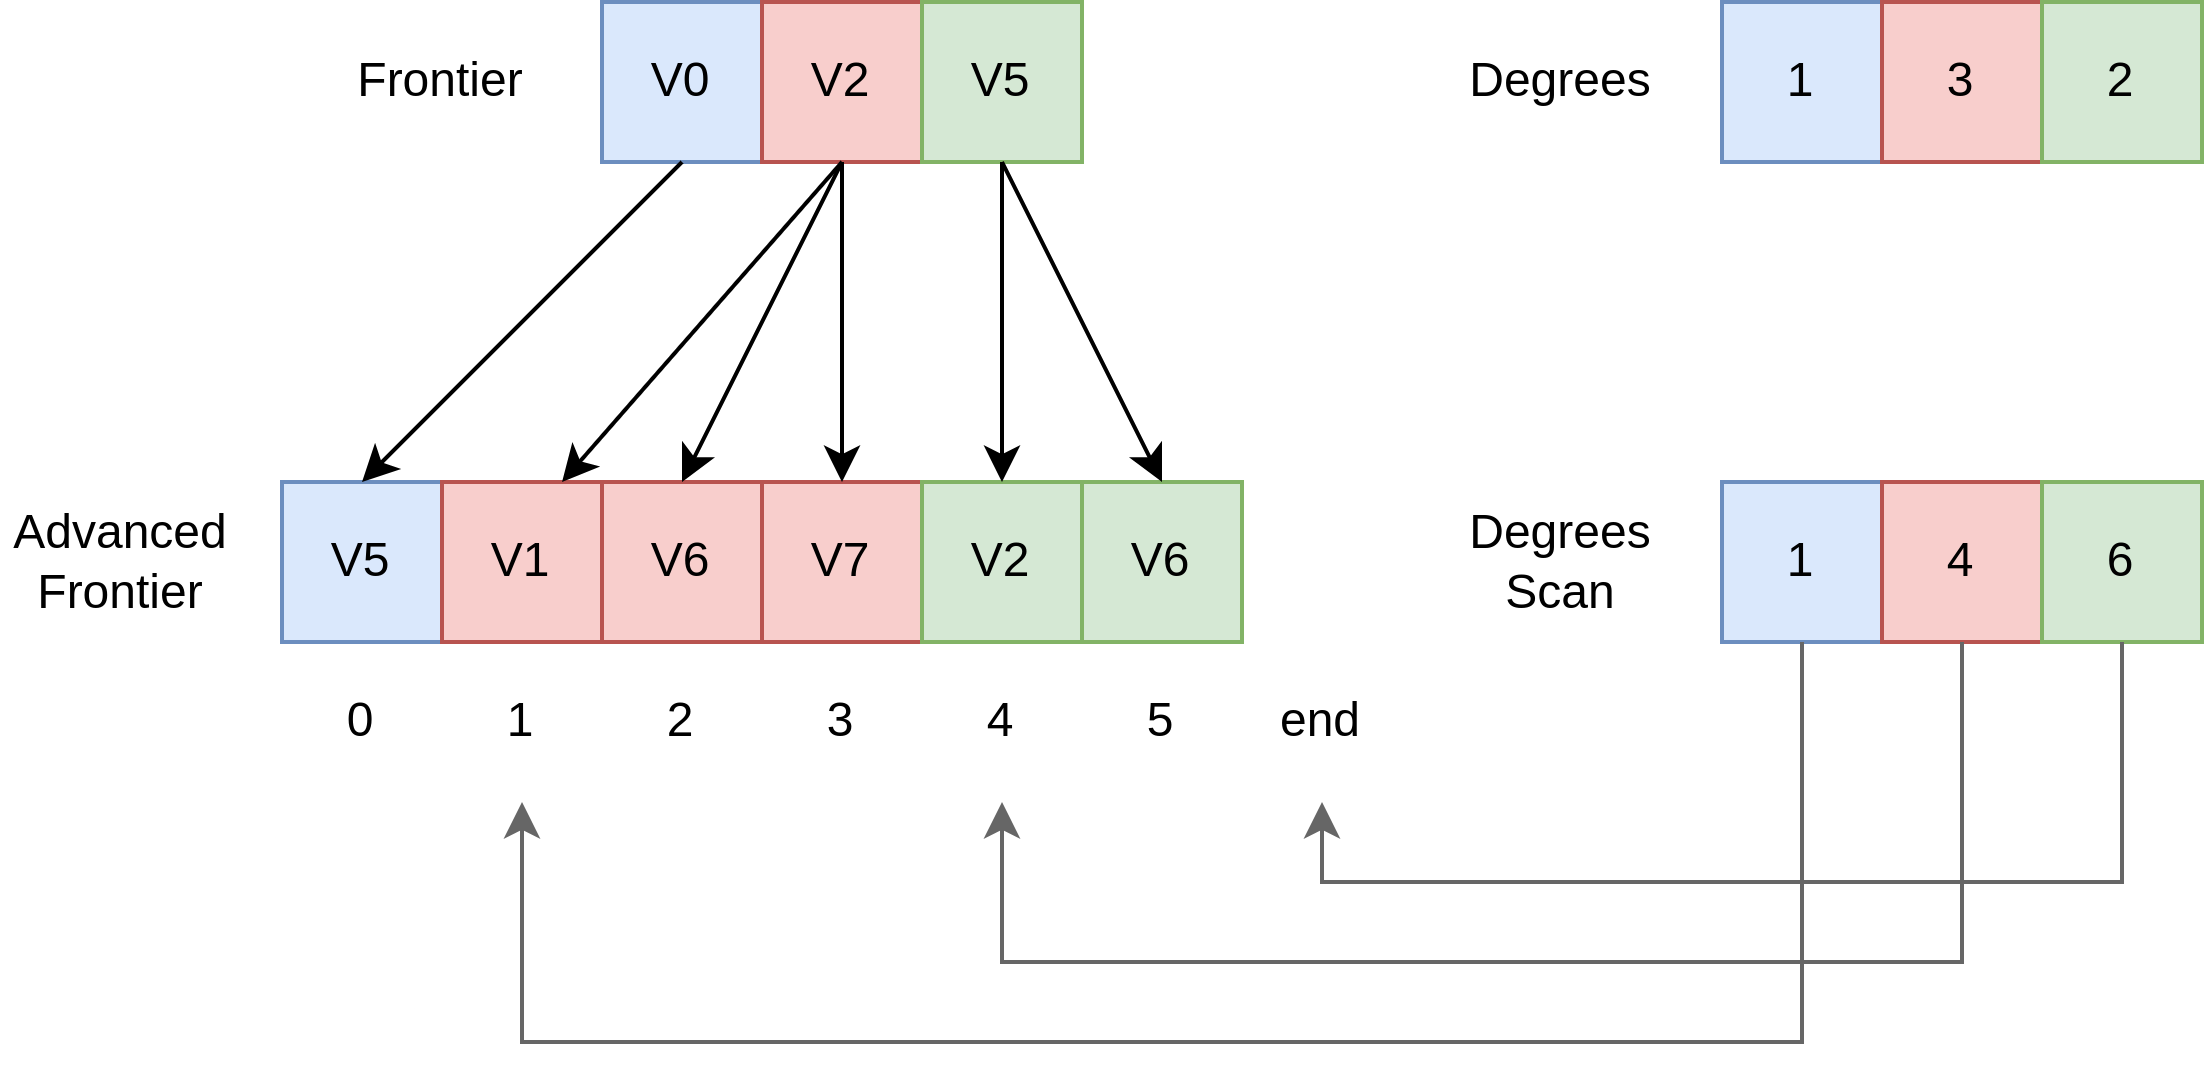
\includegraphics[width=0.8\textwidth]{Chapters/Figures/Images/af_binary_search.png}
    \caption{Advanced frontier diagram.}
\label{fig:advanced_frontier_binary_search}
\end{figure}

With the source vertex, we can now obtain the outgoing edge assigned to a thread.  We start by computing the neighbor offset (Line~18) by subtracting the degree, of the previous source vertex, from \texttt{tid}. For example, returning to Figure~\ref{fig:advanced_frontier_binary_search}, assuming \texttt{tid} is equal to $2$, the offset of the neighbor \texttt{V6} of the source vertex \texttt{V2} can be computed by subtracting the degree of the source vertex \texttt{V0} from \texttt{tid}. We can confirm that \texttt{tid} $-$ \texttt{deg(V0)} $ = 2 - 1 = 1$ is indeed the offset of \texttt{V6} in the adjacency list of \texttt{V2}. With the neighbor offset \texttt{neighbour\_n}, we can compute the block index and inner-block-offset where the edge is stored (Lines~20-22). In Lines~23-25 we iterate through the block list until we reach the desired block, and obtain the edge. In the end of the function, the destination of the edge is returned (Line~41).

Lines~28-31 update the \texttt{unique\_flags} container. Each time an outgoing edge is obtained, we atomically increment the \texttt{duplicates} value for that edge's destination vertex. If the previous value of \texttt{duplicates} is greater than $0$, i.e. there already exists an entry in the advanced frontier for that destination vertex, we set \texttt{unique\_flags} at \texttt{tid} to $0$.

In Lines~33-40, we invoke the compute operator, passing it the source vertex, destination vertex, edge, and variadic compute arguments, just like we specified in our model  (Section~\ref{sec:marrow_graph_programming_model}). Additionally, we check whether or not a \texttt{graph\_bal\_t} struct should also be passed to the compute functor (Line~33-34). As we saw in Listing~\ref{lst:segmented_intersection_example}, we sometimes need to pass this struct to the compute functor, in order to be able to use the \texttt{segmented\_intersection} function. We therefore verify what parameters the functor is expecting, and pass them accordingly.

\paragraph{\textbf{Frontier-less Advance}.}
We previously mentioned in Section~\ref{sec:marrow_graph_interface} that it is possible to invoke an optimized variant of the advance operator that does not return the advanced frontier. Let us call this variant the frontierless advance. It was also mentioned that both a balanced and unbalanced version of the frontier-less advance can be chosen. Starting with the balanced frontier-less advance, this variant operates identically to the default advance operator but does not require dealing with duplicate removal. This means that a set of instructions and device-executed operators can be omitted. In the advance Algorithm~\ref{alg:advance}, we omit the last filter (Line~6) which removes duplicates. In the advance function (Listing~\ref{lst:graph_bal_advance}), we omit Lines~8-10 which setup the \texttt{unique\_flags} and \texttt{duplicates} containers. And finally in the advance Marrow function (Listing~\ref{lst:graph_bal_advance_marrow_function}), we omit Lines~27-31 which deal with updating the \texttt{unique\_flags} and \texttt{duplicates} containers. 

Even though the balanced frontier-less advance operator allows for a significant optimization compared to the default advance operator, for sparse graphs (which should have small adjacency lists), it is possible to optimize even further. We do so in the unbalanced frontierless advance. Note that even in the balanced frontier-less advance, we perform at least four host-device communications. The first when we invoke the \texttt{graph\_bal\_get\_degrees} function (Algorithm~\ref{alg:advance}), the second when we perform a scan over those degrees, the third when we access the last element of the scan result (which is stored on the device), and the fourth when we actually execute the \texttt{graph\_bal\_advance} function. The unbalanced frontier-less advance reduces these host-device communications to a single one. The actual invocation of the advance function. Given that we do not need to generate an advanced frontier, we do not necessarily need to calculate the \texttt{advanced\_frontier\_size} (Line~3 of Algorithm~\ref{alg:advance}). We, therefore, do not compute the degrees vector (Line~1), do not perform the scan (Line~2), and do not access the scan result on the host (Line~3). Instead, we only invoke a \texttt{graph\_bal\_unbalanced\_frontierless\_advance} function. This function instantiates and invokes a Marrow function that, contrary to the default Marrow advance Marrow function, is executed by a number of threads equal to the size of the input frontier. This means that, instead of binary searching for the source vertex, each thread loops through its neighbors, and invokes the \texttt{compute} functor for each neighbor. The complete implementation of this Marrow function can be found in Listing~\ref{lst:graph_bal_unbalanced_frontierless_advance_marrow_function} of Appendix~\ref{app:listings}. 
For dense graphs that might have very long adjacency lists of widely varying sizes, this can become quite inefficient, since there will be a large load imbalance between threads. However, for sparse graphs, with potentially small adjacency lists, the reduced host-device communication can overcome the load imbalance overhead. We were able to achieve up to x8 algorithmic speedups using the unbalanced frontier-less advance, when compared to the default advance operator, and up to x1.7 algorithmic speedups using the balanced frontier-less advance.

% Test: spmv roadNet-CA
% 3 frontierless unbalanced
% 15 frontierless balanced
% 25 frontier



% \begin{listing}
\begin{minted}
[
frame=lines,
linenos,
fontsize=\scriptsize
]
{cpp}
marrow_function
idx_t binary_search(std::size_t tid, std::size_t frontier_size, std::size_t* degrees_scan) {
    int frontier_vertex_n = -1;
    int low = 0, high = frontier_size - 1;
    while (frontier_vertex_n == -1 && low <= high) {
        int mid = (low + high) / 2;
        if (tid < degrees_scan[mid] && (mid==0 || tid >= degrees_scan[mid-1]))
            frontier_vertex_n = mid;
        else if (tid < degrees_scan[mid])
            high = mid - 1;
        else
            low = mid + 1;
    }
    return frontier_vertex_n;
}
\end{minted}
\center
\caption{Graph Bal Binary Search.}
\label{lst:binary_search}
\end{listing}

\subsection{Segmented Intersection}
\label{sec:segmented_intersection}

As we already discussed Section~\ref{sec:marrow_graph_interface}, the \texttt{segmented\_intersection} is a device function that intersects the (sorted) neighbors of two input vertices (Listing~\ref{lst:segmented_intersection_function}). The function iterates through the adjacency lists of both the vertices, and whenever it encounters a shared neighbor, it increments an intersection counter and invokes the \texttt{on\_intersection} functor. At the end of the function, the counter is returned. All the necessary data to traverse the adjacency lists is accessible through the \texttt{graph} struct. Given that it is assumed that the adjacency lists of both vertices \texttt{vertex\_a} and \texttt{vertex\_b} are sorted, the function makes use of two indexers, one for each vertex's adjacency lists. It then increments both indexers if there is an intersection, otherwise, it only increments the indexer which is indexing a neighbor with a smaller vertex ID. This ensures that all possible intersections are caught, while only having to iterate through each adjacency exactly once. The full implementation of the \texttt{segmented\_intersection} device function can be found in Listing~\ref{lst:segmented_intersection} of Appendix~\ref{app:listings}.

%\begin{algorithm}[H]
    \small
    \SetAlgoLined
    \SetKwData{nintersections}{nintersections}
    \SetKwData{degreea}{degree\_a}
    \SetKwData{degreeb}{degree\_b}
    \SetKwData{blockindexa}{block\_index\_a}
    \SetKwData{blockindexb}{block\_index\_b}
    \SetKwData{offseta}{offset\_a}
    \SetKwData{offsetb}{offset\_b}
    \SetKwData{indexa}{index\_a}
    \SetKwData{indexb}{index\_b}
    \SetKwData{edgesindexa}{edges\_index\_a}
    \SetKwData{edgesindexb}{edges\_index\_b}
    \SetKwData{intersectionargs}{int\_args}
    \SetKwData{graph}{graph}
    \SetKwFunction{onintersection}{on\_intersrction}

    \KwIn{graph\_bal\_t<> graph, vertex<> vertex\_a, vertex<> vertex\_b, int\_fun on\_intersection, int\_args... int\_args}
    \KwOut{int}
    
    \BlankLine
    $\degreea \leftarrow \graph.vertices[vertex\_a.idx].degree$\;
    $\degreeb \leftarrow \graph.vertices[vertex\_b.idx].degree$\;
    $\blockindexa \leftarrow \graph.vertices[vertex\_a.idx].adjacency\_list$\;
    $\blockindexb \leftarrow \graph.vertices[vertex\_b.idx].adjacency\_list$\;
    $\nintersections, \offseta, \offsetb, \indexa, \indexb \leftarrow 0$\;

    \BlankLine
    \While{$(\indexa < \degreea \land \indexb < \degreeb)$}{
        $\edgesindexa \leftarrow \blockindexa \times \graph.block\_size + \offseta$\;
        $\edgesindexb \leftarrow \blockindexb \times \graph.block\_size + \offsetb$\;
        $neighbor\_a \leftarrow \graph.vertices[\graph.edges[\edgesindexa].dst]$\;
        $neighbor\_b \leftarrow \graph.vertices[\graph.edges[\edgesindexb].dst]$\;
        
        \BlankLine
        \If{$(neighbor\_a.idx == neighbor\_b.idx)$}{
            $nintersections \leftarrow nintersections + 1$\;
            \onintersection{$\text{vertex\_a}$, $\text{vertex\_b}$, $\text{neighbor\_a}$, $\intersectionargs \ldots$}\;
            $\indexa \leftarrow \indexa + 1$\;
            $\offseta \leftarrow \offseta + 1$\;
            $\indexb \leftarrow \indexb + 1$\;
            $\offsetb \leftarrow \offsetb + 1$\;
        }
        \ElseIf{$(neighbor\_a.idx > neighbor\_b.idx)$}{
            $\indexb \leftarrow \indexb + 1$\;
            $\offsetb \leftarrow \offsetb + 1$\;
        }
        \Else{
            $\indexa \leftarrow \indexa + 1$\;
            $\offseta \leftarrow \offseta + 1$\;
        }
        
        \BlankLine
        \If{$(\offseta \geq \graph.block\_size)$}{
            $\offseta \leftarrow 0$\;
            $\blockindexa \leftarrow \graph.block\_links[\blockindexa]$\;
        }
        \If{$(\offsetb \geq \graph.block\_size)$}{
            $\offsetb \leftarrow 0$\;
            $\blockindexb \leftarrow \graph.block\_links[\blockindexb]$\;
        }
        \KwRet \nintersections
    }
    
    \caption{Segmented Intersection}
\end{algorithm}


\section{Algorithms}
\label{sec:marrow_graph_algorithms}

Besides the basic operators, Marrow-Graph includes a suite of implemented algorithms. The algorithms that have been implemented so far are: 
%
\begin{itemize}
    \item \gls{BFS}: Traversal algorithm that starts from a given source vertex and explores all its neighbors at the present depth level before moving on to vertices at the next depth level. This algorithm is useful to find short paths between nodes (not necessarily the shortest). Some applications include network routing and web crawling.
    \item \gls{SSSP}: Algorithm that finds the shortest paths from a given source vertex to all other vertices in the graph. Marrow-Graph follows Dijkstra's implementaiton. Some applications include network routing and path-finding in robotics and video-games.
    \item \gls{TC}: Algorithm that determines the number of triangles (three nodes that are mutually connected) in a graph. This metric is useful for understanding the clustering coefficient of the graph, which provides insights into the network's topology and density.
    \item \gls{PR}: Algorithm that is used to rank the nodes in a graph based on their importance.  It assigns a score to each node, indicating its relative significance within the graph, with a node's score being tied to the number of nodes referencing it. This algorithm was originally used by Google to rank webpages.
    \item \gls{SpMV}: Algorithm that multiplies a sparse matrix (represented by the graph) with a vector. \gls{SpMV} is used in various applications including scientific computations and machine learning.
\end{itemize}
%
Most of the logic of these algorithms was based of Gunrock's implementations given that a similar programming model is used. Of course, the specific syntax to express these algorithms is quite different and is explored in Section~\ref{sec:evaluation_expressiveness}. We will not give an exhaustive description of each algorithm's implementation, but rather, will only focus on a subset that we found worth discussing.

\subsection{SSSP}

We start by presenting the \gls{SSSP} algorithm, as it follows the most common algorithmic pattern, of advancing and filtering a frontier until it is empty while updating problem data during each advance phase. The \texttt{sssp} function (Listing~\ref{lst:sssp_function}) starts by initializing a set of Marrow vectors. A \texttt{distances} vector to store the result of the algorithm, and two \texttt{visited} and \texttt{revisit} vectors to track already visited vertices. The \texttt{dist\_fill} functor used In Line~5, fills all the elements of the container with the \texttt{FLT\_MAX} value, except for the \texttt{source} index, which is set to $0$. In Lines~11-12 we instantiate the compute and filter functors, and In Lines~13-14 we create a frontier with a single vertex, the input source vertex. The actual algorithm (Lines~16-20), runs until the frontier is empty (Line~16). In each iteration, we advance the frontier with the \texttt{sp} functor, and filter the advanced frontier with the \texttt{rm} functor. The \texttt{distances} container is wrapped as a \texttt{result} given that it is computed during the compute function, and might later be accessed by the host. Finally, once the frontier is empty, the \texttt{distances} vector is returned.

\begin{listing}
\begin{minted}
[
frame=lines,
linenos,
fontsize=\scriptsize
]
{cpp}
vector<float> sssp(graph_bal<vertex_attributes, edge_attributes> &graph, idx_t source) {

    auto nvertex = graph.get_number_of_vertex();
    vector<float> distances(nvertex);
    distances.fill_on_device(dist_fill(source));
    vector<int> visited(nvertex);
    visited.fill_on_device(0);
    vector<int> revisit(nvertex);
    visited.fill_on_device(0);

    shortest_path<vertex_attributes, edge_attributes> sp;
    remove_completed_paths<vertex_attributes> rm;
    vector<idx_t> frontier;
    frontier.push_back(source);

    while (frontier.size() != 0) {
        vector<int> advanced_frontier = graph.advance(frontier, sp, result(distances), visited, revisit);
        vector<int> filtered_frontier = graph.filter(advanced_frontier, rm, visited, revisit);
        frontier = filtered_frontier;
    }
    return distances;
}
\end{minted}
\center
\caption{SSSP function.}
\label{lst:sssp_function}
\end{listing}



The compute functor \texttt{shortest\_path} can be found in Listing~\ref{lst:sssp_compute}. The compute operator is executed over every edge traversed during the advance of a frontier. This means that during every \texttt{shortest\_path} compute function, we update the distances vector, taking into account the weights of the edges being traversed. We start by calculating the new total distance to the neighbor (the destination vertex of the traversed edge) In Line~6. We then set the distance to that neighbor as the min value between the distance that is already computed, and the new distance we calculated (Line~7). We update the \texttt{visited} vector to signal that this source vertex has been visited (Line~10), and, in case the newly calculated distance has replaced the old distance to the neighbor vertex, we mark the neighbor vertex to be revisited (Line~11-12). Given that there is a new shortest path to \texttt{dst}, we must reconsider this vertex in the next iteration.

\begin{listing}[t]
\begin{minted}
[
frame=lines,
linenos,
fontsize=\scriptsize
]
{cpp}
template <typename vertex_attributes, typename edge_attributes>
struct shortest_path {
    marrow_function void operator()(vertex<vertex_attributes>& src, vertex<vertex_attributes>& dst, 
      edge<edge_attributes>& edge, float *distances, int *visited, int *revisit) {

        float distance_to_neighbor = distances[src.idx] + edge.attributes.weight;
        marrow::atomic::min(&distances[dst.idx], distance_to_neighbor);
        float recover_distance = distances[dst.idx];

        marrow::atomic::exch(&visited[src.idx], 1);
        if (recover_distance == distance_to_neighbor)
            marrow::atomic::exch(&revisit[dst.idx], 1);
    }
} ;
\end{minted}
\center
\caption{SSSP compute function.}
\label{lst:sssp_compute}
\end{listing}



The filter functor \texttt{remove\_completed\_paths} can be found in Listing~\ref{lst:sssp_filter}. It starts by checking if the degree of the source vertex is $0$, in which case, it can be excluded from the filtered frontier (Line~5-6). This is not necessary for the correctness of the algorithm, but makes it slightly more efficient, given that neighbor-less vertices will not have any impact in the advance phase. We then check if the vertex has been marked for a revisit (Line~8), in which case, we set both the visited and revisit flags to $0$. Finally, we include the vertex from the filtered frontier if the visited flag is set to $0$, otherwise, the vertex is excluded. This ensures that we do not revisit vertices that have already been visited, and whose shortest distance has not been updated in the last advance phase. Additionally, this ensures that the frontier converges to empty, which is necessary for the algorithm loop to end.

\begin{listing}[t]
\begin{minted}
[
frame=lines,
linenos,
fontsize=\scriptsize
]
{cpp}
template <typename vertex_attributes>
struct remove_completed_paths {
    marrow_function int operator()(vertex<vertex_attributes>& v, int *visited, int *revisit) {

        if(v.degree == 0)
            return 0;

        if(revisit[v.idx]) {
            marrow::atomic::exch(&revisit[v.idx], 0);
            marrow::atomic::exch(&visited[v.idx], 0);
        }
        return visited[v.idx] ? 0 : 1;
    }
};
\end{minted}
\center
\caption{SSSP filter function.}
\label{lst:sssp_filter}
\end{listing}


\subsection{Triangle Count} 

We now present the \gls{TC} algorithm given it is the main application and motivator for the segmented intersection function. The \texttt{tc} function (Listing~\ref{lst:tc_function}) starts by initializing a vector to store the triangle counts of all the vertices (the result), with all values set to $0$. We then initialize a frontier that contains the IDs of all the vertices of the graph. Assuming there are no deleted vertices, we can do so using the \texttt{iota} function that generates a vector of $N$ counting integers $[0, 1, 2, \ldots, N]$. 
% We then obtain the frontier that contains the IDs of all the vertices of the graph using the provided \texttt{all\_vertices} function.
In Lines~8-9 we instantiate the compute functor \texttt{trig\_count} and the on intersection functor \texttt{trig\_count\_seg}. In Line~11 we perform a single advance over the frontier containing all the vertices in the graph, which computes the triangle count for each one. Since we do not require the resulting advanced frontier, we call the optimized unbalanced frontier-less advance operator, by setting the corresponding boolean templates to false.
%In Line~12 we dirty the \texttt{vertex\_triangle\_count} vector's replica (for the same reasons described in Section~\ref{sec:host_dev_sync}). 
Finally, In Line~12-13, we sum all the triangle counts with a Marrow reduce, and return the result. Note that the result is divided by $3$. Because the \texttt{triangle\_count} stores, for each vertex $v$, the number of triangles in the graph that include $v$, we must divide the total sum of triangle counts by the number of vertices in a triangle, i.e. $3$.

\begin{listing}
\begin{minted}
[
frame=lines,
linenos,
fontsize=\scriptsize
]
{cpp}
int tc(graph_bal<vertex_attributes, edge_attributes> &graph) {

    auto nvertex = graph.get_number_of_vertex();
    vector<int> vertex_triangle_count(nvertex);
    vertex_triangle_count.fill_on_device(0);
    vector<idx_t> frontier = iota(nvertex);

    triangle_count_fun<vertex_attributes, edge_attributes> trig_count;
    on_intersection_fun<vertex_attributes> trig_count_seg;

    graph.advance<false,false>(frontier, trig_count, trig_count_seg, vertex_triangle_count);
    int tcount = reduce<sum<int>>(vertex_triangle_count) / 3;
    return tcount;
}
\end{minted}
\center
\caption{TC Function.}
\label{lst:tc_function}
\end{listing}

The compute functor \texttt{triangle\_count\_fun} can be found in Listing~\ref{lst:tc_compute}. We omitted the functor's parameters for conciseness. As we can see, the only thing the functor does is call the \texttt{segmented\_intersection} function. It passes all the necessary parameters, but most importantly, passes the \texttt{on\_intersec} functor, which contains all the important logic of the algorithm, and the \texttt{vertex\_triangle\_count} container that is manipulated in \texttt{on\_intersec}. The only logic that is present in the compute functor, is the conditional statement (Line~4), which prevents the algorithm from counting repeated triangles. Given that this algorithm is implemented for undirected graphs, the same triangle can be counted twice in each direction. We prevent this by only considering triangles in the direction of ascending indices.

\begin{listing}
\begin{minted}
[
frame=lines,
linenos,
fontsize=\scriptsize
]
{cpp}
template <typename vertex_attributes, typename edge_attributes>
struct triangle_count_fun {
    marrow_function void operator()(/*...*/) {
        if(dst.idx > src.idx) {
            segmented_intersection(graph, src, dst, on_intersec, vertex_triangle_count);
        }
    }
};
\end{minted}
\center
\caption{TC compute function.}
\label{lst:tc_compute}
\end{listing}

The on intersection functor \texttt{on\_intersection\_fun} can be found in Listing~\ref{lst:tc_on_intersection}. The function starts by checking whether the intersection \texttt{intersection\_vertex} does not coincide with one of the intersecting vertices \texttt{vertex\_a} or \texttt{vertex\_b}. If not, the triangle count of the intersection vertex is incremented atomically. 

To clarify why this works, we present an example using Figure~\ref{fig:trig_count_example}. Looking at this undirected graph, it is obvious that it contains $3$ triangles. When we perform an advance over the frontier containing all the vertices in the graph, we are essentially traversing all the edges of the graph. We can see that when we traverse, for example, the edge $\{V_0, V_4\}$, a segmented intersection is performed between these two vertices, resulting in a single intersection (a single neighbor in common) $V_1$. With this, the triangle count of $V_1$ is incremented to $1$. This count is incremented again in the traversal of edge $\{V_0, V_2\}$, since $V_1$ is also a common neighbor between these vertices. This results in a total triangle count of $2$, like we can see in the figure. Turning our attention to vertex $V_4$, we can see it has a total triangle count of just $1$. The traversal of edge $\{V_0, V_1\}$ results in a \texttt{tc} increment for $V_4$ (since $V_4$ is a common neighbor of $V_0$ and $V_1$), but the traversal of the edge $\{V_1, V_0\}$ does not. It does not because $V_0$ has a lesser ID than $V_1$, and In Line~4 of Listing~\ref{lst:tc_compute}, we can see that we only perform segmented intersections between edges whose destination vertex ID is greater than the source vertex's ID. In practice, each vertex ends up with a triangle count equal to the number of triangles that include that specific vertex. $V_4$ is part of a single triangle, $V_1$ is part of two triangles, $V_0$ is part of three triangles, etc. If we sum all the triangle counts and divide them by $3$, we get $(3+2+2+1+1)/3=3$, the number of triangles in the graph.

\begin{listing}
\begin{minted}
[
frame=lines,
linenos,
fontsize=\scriptsize
]
{cpp}
template <typename vertex_attributes>
struct on_intersection_fun {
    marrow_function int operator()(
      vertex<vertex_attributes>& vertex_a,
      vertex<vertex_attributes>& vertex_b,
      vertex<vertex_attributes>& intersection_vertex,
      int* vertex_triangle_count) {

        if (vertex_a.idx != intersection_vertex.idx && vertex_b.idx != intersection_vertex.idx) {
            marrow::atomic::add( &(vertex_triangle_count[intersection_vertex.idx]), 1);
        }
    }
};
\end{minted}
\center
\caption{TC on intersection function.}
\label{lst:tc_on_intersection}
\end{listing}

\begin{figure}
  \centering
    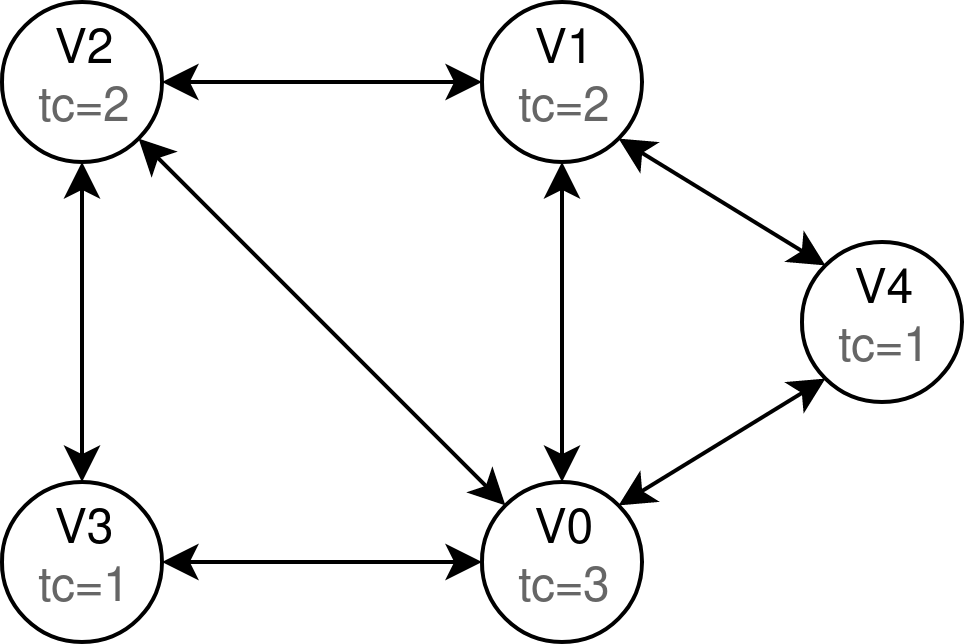
\includegraphics[width=0.4\textwidth]{Chapters/Figures/Images/triangle_count.png}
    \caption{Triangle count example.}
\label{fig:trig_count_example}
\end{figure}





\section{Marrow Adaptation}

Due to some technical challenges with Marrow during the development of this thesis, an adapted and simplified runtime was developed and used to implement Marrow-Graph. Because of time constraints, we were not able to run our solution on the original and complete version of Marrow. This is something we would like to tackle in future work. Nevertheless, the solution is working correctly and showing promising results. In this section, we present the differences and relevant technical details regarding the adaptation, which we will call \textit{lmarrow}.

\textit{lmarrow}'s syntax is a direct subset of Marrow's, supporting the main smart containers: \texttt{array}, \texttt{vector}, \texttt{vector<array>} and \texttt{scalar}, the main skeletons: \texttt{map}, \texttt{filter}, \texttt{reduce} and \texttt{scan}, and the same generic \texttt{function} primitive. Just like Marrow, \textit{lmarrow} allocates and synchronizes the smart containers automatically in a lazy manner, and executes the skeletons and functions on the device.
%
The main differences in the adaptation are:
\begin{enumerate}
    \item The lack of Marrow-expressions, meaning that skeletons always return the resulting containers and not the corresponding expression. Therefore, skeleton composition is not supported.
    \item The lack of a scheduler that manages the execution of kernels asynchronously and deals with data dependencies. \textit{lmarrow} invokes most device operations sequentially on the default stream.
    \item \textit{lmarrow} only supports CUDA, and does not include multiple backends.
\end{enumerate}

For the specific needs of Marrow-Graph, these drawbacks fortunately are not too concerning in terms of performance. Regarding the first, Marrow-Graph does not directly make use of skeleton composition. Regarding the second, given the bulk-synchronous nature of Marrow-Graph's programming model, the potential for asynchronous kernel management is limited (although not nonexistent). Regarding the third, we planned on only using the CUDA backend during this thesis.

Given the aim of this thesis, we will not give a detailed description of \textit{lmarrow}'s implementation. Additionally, since we plan to eventually run our solution on the original complete version of Marrow, we left all the code ready to be run on the non-adapted library. For example, we used the \texttt{auto} keyword whenever a Marrow expression can be captured instead of a container. This means that while using \textit{lmarrow}, these variable types will be containers, but once Marrow is integrated, these variables will be typed with the lighter-weight Marrow expressions. For the rest, from a user perspective, every thing stays the same, and almost all information provided in Section~\ref{sec:marrow} is still relevant.